% This template is created by SV Bùi Vân Anh, và Thầy Nguyễn Tiến Hòa từ phòng Lab xử lý tín hiệu băng gốc hệ thống 5G. Chúng tôi rất vui nếu được nhắc đến trong lời cảm ơn.
%%%%%%%%%%%%%%%%%%%%%%%%%%%%%%%%%%%%%%%%%%%%%%%%%%%%%%%
\documentclass{article} % Tạo một bản báo cáo
\usepackage[utf8]{inputenc}
\usepackage[T5]{fontenc} % Để sử dụng Tiếng Việt
\usepackage[fontsize=13pt]{scrextend} % Set fontsize=13pt
%\usepackage[paperheight=29.7cm,paperwidth=21cm,right=2cm,left=3cm,top=2cm,bottom=2.5cm]{geometry}% Chuẩn A4, căn lề phải, trái, trên, dưới.
\usepackage[paperheight=29.7cm,paperwidth=21cm,right=2cm,left=3cm,top=2cm,bottom=2.5cm,twoside]{geometry}% Chuẩn A4, căn lề phải, trái, trên, dưới.
\usepackage{mathptmx} % Time New Roman
\usepackage{listings}
\usepackage{xcolor}
\usepackage{amsmath}
\usepackage{longtable}
\usepackage{geometry}
\usepackage{array}
\usepackage{url}
\usepackage{xcolor}
\usepackage{graphicx} % Thư viện chèn ảnh
\usepackage{float} % Set vị trí chèn ảnh
\usepackage{tikz} % Thư viện tạo khung bìa
\usepackage{forest}
\usepackage{enumitem}  % cho phép cấu hình danh sách
\usepackage[utf8]{inputenc}
\usepackage{newunicodechar}
\newunicodechar{≈}{\approx}
\setlist[itemize]{                 % cấu hình mặc định cho TẤT CẢ itemize
  leftmargin=2.5em,               % lùi cả bullet + nội dung 2.5 em
  labelsep=0.6em,                 % khoảng cách giữa bullet và chữ
  topsep=0.2em,                   % thu hẹp khoảng trắng trước / sau list
  itemsep=0.2em                   % thu hẹp khoảng trắng giữa các item
}
\setlist[enumerate]{leftmargin=2.5em,labelsep=0.6em,topsep=0.2em,itemsep=0.2em}
\forestset{
  default preamble={
    font=\ttfamily\small,
    grow'=0,
    child anchor=west,
    parent anchor=east,
    edge={-},
    l sep=1cm,
    s sep=2mm
  }
}
\tikzset{
    box/.style={draw, rounded corners=2pt,
               minimum width=28mm, minimum height=10mm,
               align=center, inner sep=2pt},
  innerbox/.style={draw, rounded corners=2pt, fill=gray!12,
                   minimum width=25mm, minimum height=8mm,
                   align=center, inner sep=2pt},
  arrow/.style={-{Stealth[scale=0.9]}, thick}
}
\lstdefinelanguage{bash}{
  keywords={make, all},
  keywordstyle=\color{blue}\bfseries,
  sensitive=true,
  morecomment=[l]{\#},
  commentstyle=\color{gray}\ttfamily,
  morestring=[b]",
}

\lstset{
  basicstyle=\ttfamily\small,
  breaklines=true,
  language=bash,
  frame=single,
  backgroundcolor=\color{gray!10},
  captionpos=b
}
\usetikzlibrary{
  positioning, shapes.geometric, shapes.multipart,
  fit, arrows.meta, backgrounds, matrix
}
\usetikzlibrary{calc} % Thư viện tikz
\usepackage{indentfirst} % Thư viện thụt đầu dòng
\usepackage{booktabs} % To thicken table lines
\renewcommand{\baselinestretch}{1.2} % Giãn dòng 1.2
\setlength{\parskip}{6pt} % Spacing after
\setlength{\parindent}{1cm} % Set khoảng cách thụt đầu dòng mỗi đoạn
\usepackage{titlesec} % Thư viện để set up các kiểu chữ
\setcounter{secnumdepth}{4} % 4 Heading
\titlespacing*{\section}{0pt}{0pt}{30pt} % Heading 1
\titleformat*{\section}{\fontsize{16pt}{0pt}\selectfont \bfseries \centering}

\titlespacing*{\subsection}{0pt}{10pt}{0pt} % Heading 2
\titleformat*{\subsection}{\fontsize{14pt}{0pt}\selectfont \bfseries}

\titlespacing*{\subsubsection}{0pt}{10pt}{0pt} % Heading 3
\titleformat*{\subsubsection}{\fontsize{13pt}{0pt}\selectfont \bfseries \itshape}

\titlespacing*{\paragraph}{0pt}{10pt}{0pt} % Heading 4
\titleformat*{\paragraph}{\fontsize{13pt}{0pt}\selectfont \itshape}

\renewcommand{\figurename}{\fontsize{12pt}{0pt}\selectfont \bfseries Figure}
\renewcommand{\thefigure}{\thesection.\arabic{figure}}
\usepackage[font=bf]{caption}
\captionsetup[figure]{labelsep=space}

\renewcommand{\tablename}{\fontsize{12pt}{0pt}\selectfont \bfseries Table}
\renewcommand{\thetable}{\thesection.\arabic{table}}
\captionsetup[table]{labelsep=space}

\usepackage{tabularx}
\newcolumntype{s}{>{\hsize=.3\hsize}X}
\newcolumntype{y}{>{\hsize=.4\hsize}X}
\newcolumntype{d}{>{\hsize=.1\hsize}X}
\newcolumntype{a}{>{\hsize=1.1\hsize}X}
\newcolumntype{g}{>{\hsize=5\hsize}X}
\renewcommand{\tabularxcolumn}[1]{>{\small}m{#1}}

\renewcommand{\theequation}{\thesection.\arabic{equation}} % Thay đổi đánh số phương trình mặc định
\newtheorem{theorem}{Định lý}[section]
\newtheorem{defn}[theorem]{Định nghĩa}
\newtheorem{corollary}[theorem]{Hệ quả}
\newtheorem{lemma}[theorem]{Bổ đề}

\usepackage{lipsum} % Thư viện tạo chữ linh tinh.
\renewcommand{\contentsname}{TABLE OF CONTENTS}
\renewcommand{\listfigurename}{LIST OF FIGURES}
\renewcommand{\listtablename}{LIST OF TABLES}
\renewcommand{\lstlistlistingname}{LIST OF LISTINGS}
\renewcommand{\refname}{REFERENCES}

\usepackage[unicode]{hyperref}
\renewcommand{\theHfigure}{\thesection.\arabic{figure}}
\renewcommand{\theHtable}{\thesection.\arabic{table}}
\renewcommand{\theHequation}{\thesection.\arabic{equation}}
\usepackage{colortbl}
\definecolor{LightCyan}{rgb}{0.88,1,1}
\usepackage{forloop}
\newcounter{loopcntr}
\newcommand{\rpt}[2][1]{\forloop{loopcntr}{0}{\value{loopcntr}<#1}{#2}}

\begin{document}
\hypersetup{pageanchor=false}

\begin{titlepage}
\thispagestyle{empty}

% ===== Border =====
\begin{tikzpicture}[overlay,remember picture]
\draw [line width=3pt]
    ($ (current page.north west) + (3.0cm,-2.0cm) $)
    rectangle
    ($ (current page.south east) + (-2.0cm,2.5cm) $);

\draw [line width=0.5pt]
    ($ (current page.north west) + (3.1cm,-2.1cm) $)
    rectangle
    ($ (current page.south east) + (-2.1cm,2.6cm) $); 
\end{tikzpicture}

\begin{center}

% ===== Header =====
\vspace*{-0.3cm}

{\fontsize{13pt}{16pt}\selectfont HANOI UNIVERSITY OF SCIENCE AND TECHNOLOGY}
\resizebox{0.88\textwidth}{!}{
    \textbf{SCHOOL OF ELECTRICAL AND ELECTRONIC ENGINEERING}
}

% ===== Logo =====
\vspace{1.8cm}


\includegraphics[width=3cm]{Images/logodhbk.png}

% ===== Main title =====
\vspace{2.0cm}

{\fontsize{26pt}{32pt}\selectfont\textbf{GRADUATION THESIS}}

% ===== Thesis title =====
\vspace{1.6cm}

{\fontsize{18pt}{23pt}\selectfont\textbf{
SIMULATION-BASED 5G RADIO MEASUREMENT\\[0.2cm]
DATA GENERATION AND LOG-BASED\\[0.2cm]
HANDOVER DELAY ANALYSIS
}}

% ===== Student information =====
\vspace{2.0cm}

\begin{tabular}{ll}
\textbf{\fontsize{14pt}{17pt}\selectfont Student:} 
& {\fontsize{14pt}{17pt}\selectfont Hoang Gia Duc} \\

\textbf{\fontsize{14pt}{17pt}\selectfont ID:} 
& {\fontsize{14pt}{17pt}\selectfont 20224339} \\

\textbf{\fontsize{14pt}{17pt}\selectfont Class:} 
& {\fontsize{14pt}{17pt}\selectfont ET-E4 01 K67} \\
\end{tabular}

% ===== Supervisor =====
\vspace{1.8cm}

\begin{tabular}{ll}
\textbf{\fontsize{14pt}{17pt}\selectfont Supervisor:} 
& {\fontsize{14pt}{17pt}\selectfont Dr. Phung Thi Kieu Ha}
\end{tabular}

% ===== Date =====
\vfill

{\fontsize{13pt}{16pt}\selectfont Hanoi, \today}

\vspace{0.3cm}

\end{center}

\end{titlepage}

\cleardoublepage
 % Bìa đồ án.

\input{DanhGia} % Đánh giá quyển đồ án tốt nghiệp cho giảng viên hướng dẫn và cán bộ phản biện.

\section*{PREFACE}
\thispagestyle{empty}
% Bối cảnh và tầm quan trọng của lĩnh vực: Giới thiệu lĩnh vực nghiên cứu  Cho thấy vì sao chủ đề này quan trọng

% Nêu vấn đề: Chỉ ra khoảng trống hoặc khó khăn  -->  Trả lời câu hỏi: "Tại sao cần làm đề tài này?"

% Giải pháp và đóng góp: Đề tài làm gì Phương pháp gì Đóng góp gì

% Lời cảm ơn


As fifth-generation (5G) mobile networks continue to expand, mobility management has become an important aspect of maintaining service continuity and network performance. Among mobility procedures, handover plays a key role because user equipment may need to move between serving cells while radio conditions and network conditions change over time. This topic is important not only from the viewpoint of radio coverage, but also from the viewpoint of signaling procedures and timing behavior inside the network.

However, collecting detailed 5G mobility data in real environments is difficult because measurement campaigns require suitable equipment, stable test conditions, and repeated experiments. In addition, handover behavior cannot be fully understood from radio measurements alone, since a change in the best serving cell does not necessarily mean that the protocol-level handover procedure has been completed. These difficulties motivated the development of a controlled study environment in which radio measurements and handover-delay behavior can be inspected more systematically.

For that reason, this graduation thesis was developed to support the study of 5G mobility through simulation-based radio-data generation and log-based handover-delay analysis. The work focuses on generating structured radio-measurement data and examining handover delay from timer-event logs under different timer configurations and network-condition settings.

Through this work, radio-level serving-cell decisions and protocol-level handover completion can be considered separately. This separation provides a clearer basis for observing handover behavior and for evaluating how timer configurations and network conditions may influence completion time, timeout cases, and failure behavior.

I would like to express my deepest gratitude to \textbf{Dr. Phung Thi Kieu Ha} for her guidance, feedback, and support throughout this graduation thesis. I also thank the lecturers of the School of Electrical and Electronic Engineering, Hanoi University of Science and Technology, for providing the technical and academic foundation necessary for this work. Due to limitations in time, experimental resources, and experience, some limitations may remain. I sincerely welcome constructive comments and suggestions that can improve both the thesis and the research platform.

\clearpage
 % Lời nói đầu.

\section*{DECLARATION OF AUTHORSHIP}
\thispagestyle{empty}
I am Hoang Gia Duc, student ID 20224339, a student of the Advanced Program in Electronics and Telecommunication Engineering, cohort K67. I declare that the thesis entitled "\textbf{Simulation-Based 5G Radio Measurement Data Generation and Log-Based Handover Delay Analysis}" was carried out by myself under the supervision of \textbf{Dr. Phung Thi Kieu Ha}. All data, results, and evaluations presented in this thesis are reported honestly and reflect the actual outcomes obtained during the research process. All referenced documents, source code, standards, and technical materials have been properly cited and listed in accordance with academic and intellectual property regulations. I take full responsibility for the content of this thesis.

\vspace{6pt}

\begin{flushright}
\begin{minipage}{6cm}
\centering
Hanoi, \today

\vspace{12pt}

\textbf{Author}

\vspace{4pt}

\includegraphics[width=4cm]{Images/signature.png}

\vspace{4pt}

\textbf{Hoang Gia Duc}
\end{minipage}
\end{flushright}

\clearpage
 % Lời cam đoan.

 % Tạo mục lục tự động
\addtocontents{toc}{\protect\thispagestyle{empty}}
\tableofcontents 
\thispagestyle{empty}
\cleardoublepage

\cleardoublepage
\pagenumbering{roman}
\hypersetup{pageanchor=true}
\section*{ABBREVIATIONS}
\phantomsection\addcontentsline{toc}{section}{\protect\numberline{}ABBREVIATIONS}

\begin{longtable}{p{2.8cm}p{11.2cm}}
3GPP & Third Generation Partnership Project\\
5G & Fifth Generation\\
5GC & 5G Core\\
A2G & Air-to-Ground\\
AMF & Access and Mobility Management Function\\
BS & Base Station\\
CHO & Conditional Handover\\
CSV & Comma-Separated Values\\
DL & Downlink\\
eMBB & enhanced Mobile Broadband\\
FSM & Finite-State Machine\\
gNB & next-generation NodeB\\
GTP-U & GPRS Tunnelling Protocol for the User Plane\\
HO & Handover\\
HOM & Handover Margin\\
ISD & Inter-Site Distance\\
LOS & Line-of-Sight\\
mMTC & massive Machine-Type Communications\\
N2 & Control-plane interface between a gNB and the AMF\\
N3 & User-plane interface between a gNB and the UPF\\
NAS & Non-Access Stratum\\
NGAP & NG Application Protocol\\
NLOS & Non-Line-of-Sight\\
NTN & Non-Terrestrial Network\\
PDU & Protocol Data Unit\\
PLMN & Public Land Mobile Network\\
RAN & Radio Access Network\\
RB & Resource Block\\
RLF & Radio Link Failure\\
RRC & Radio Resource Control\\
RSRP & Reference Signal Received Power\\
SCTP & Stream Control Transmission Protocol\\
SINR & Signal-to-Interference-plus-Noise Ratio\\
SMF & Session Management Function\\
TN & Terrestrial Network\\
UAV & Unmanned Aerial Vehicle\\
UE & User Equipment\\
UL & Uplink\\
UPF & User Plane Function\\
URLLC & Ultra-Reliable Low-Latency Communications\\
Xn & Logical interface between gNBs\\
\end{longtable}

\newpage
 % Danh mục ký hiệu và chữ viết tắt

%Tạo danh mục hình vẽ.
{\let\oldnumberline\numberline
\renewcommand{\numberline}{Figure~\oldnumberline}
\listoffigures} 
\phantomsection\addcontentsline{toc}{section}{\protect\numberline{} LIST OF FIGURES}
\newpage

%Tạo danh mục bảng biểu.
{\let\oldnumberline\numberline
\renewcommand{\numberline}{Table~\oldnumberline}
\listoftables}
\phantomsection\addcontentsline{toc}{section}{\protect\numberline{} LIST OF TABLES}
\newpage

%Tạo danh mục List code.
{\let\oldnumberline\numberline
\renewcommand{\numberline}{Table~\oldnumberline}
\lstlistoflistings}
\phantomsection\addcontentsline{toc}{section}{\protect\numberline{} LIST OF LISTINGS}
\newpage

\section*{ABSTRACT}
\phantomsection\addcontentsline{toc}{section}{\protect\numberline{}ABSTRACT}

This thesis investigates mobility behavior in fifth-generation (5G) networks through radio-measurement data generation and handover-delay analysis. Since real-world 5G measurement campaigns require specialized equipment, repeated field tests, and stable experimental conditions, collecting detailed mobility datasets remains challenging. In addition, handover performance cannot be evaluated only from serving-cell changes, because a radio-level decision does not necessarily indicate the completion of the protocol-level handover procedure.

To address these issues, this thesis develops a simulation-based radio-data generation workflow and a log-based handover-delay analysis workflow. The first part generates structured 5G radio-measurement data during UE movement, including mobility information, serving-cell changes, radio-channel characteristics, and handover-related indicators. The second part analyzes handover delay using timer-event logs under different timer configurations and network-condition settings.

The proposed workflow separates radio-level serving-cell decisions from protocol-level handover completion. This separation enables clearer observation of handover behavior and provides a basis for evaluating completion time, timeout cases, failure behavior, and recovery margin. The results show that timer configuration and network conditions have an important influence on handover performance, especially in cases where signaling delay or packet loss affects the completion process.

Overall, this thesis provides a practical platform for generating 5G mobility data and analyzing handover delay beyond simple success-or-failure outcomes. The workflow can support further experiments on mobility optimization, timer configuration, and data-driven handover analysis.

\cleardoublepage
 % Tóm tắt đồ án 

\pagenumbering{arabic} % Đánh số thứ tự 1,2,3...
\section*{CHAPTER 1. INTRODUCTION}
\addcontentsline{toc}{section}{\protect\numberline{}CHAPTER 1. INTRODUCTION}
\setcounter{section}{1}
\setcounter{subsection}{0}
\setcounter{figure}{0}
\setcounter{table}{0}
\subsection{Research Context}

Mobility management is an essential function in 5G networks because user equipment (UE) is expected to maintain service continuity while moving through an environment with continuously changing radio conditions. In a mobile scenario, the radio link between a UE and surrounding gNBs is not fixed. As the UE changes its position or height, the distance to each gNB, the line-of-sight (LOS) condition, the path loss, the shadow fading component, and the interference level can all vary over time. These variations directly affect radio measurements such as reference signal received power (RSRP), received signal strength, and signal-to-interference-plus-noise ratio (SINR). Since these measurements are commonly used to evaluate serving-cell quality, they provide an important basis for cell selection, cell reselection, and handover-related decisions.

In dense 5G deployments, this problem becomes more significant because the UE may observe several candidate cells with comparable signal quality. A small change in position may improve the received signal from one gNB while reducing the quality of another. Similarly, a temporary obstruction or a rapid change in interference may cause the best serving-cell candidate to change within a short time interval. If mobility decisions are made too late, the UE may experience degraded signal quality before the handover is completed. If they are made too aggressively, unnecessary handovers may occur, increasing signaling overhead and possibly causing instability. Therefore, studying mobility behavior requires not only observing the final serving cell, but also understanding how the underlying radio measurements evolve before, during, and after a potential handover event.

At the same time, handover is not only a radio-measurement problem. Radio measurements may indicate that a target cell is more suitable, but the actual handover still requires a protocol procedure involving the source gNB, target gNB, UE, and 5G core network (5GC). After the target cell is selected, signaling messages must be exchanged, resources must be prepared, and timers must be monitored until the procedure either completes successfully or fails. The final handover delay can therefore be affected by transport latency, packet loss, jitter, and protocol timer configuration. For this reason, a complete study of mobility should consider both radio-level measurements and protocol-level handover execution. The radio layer explains why a serving-cell change may be needed, while the protocol layer explains how long the handover procedure takes and whether it can complete under the given network conditions.

\subsection{Problem Statement}

Detailed 5G mobility datasets are not always available for controlled research. Real measurement campaigns require suitable radio equipment, repeated field tests, consistent scenarios, and considerable time and effort. In practice, it is difficult to repeat the same UE movement path, the same propagation condition, and the same network configuration many times while changing only one parameter of interest. Environmental factors such as obstacles, traffic load, interference, and user movement may also change between test runs. As a result, real-world measurement data is valuable, but it is not always convenient for isolating the influence of individual radio factors.

Public or archived datasets may also miss intermediate radio parameters, serving-cell decisions, or handover-related labels. Some datasets provide final throughput or connection status, but do not include enough detail about path loss, shadow fading, per-cell RSRP, SINR, or the exact condition that caused a serving-cell change. Other datasets may contain radio measurements but may not include handover indicators or protocol-level information. This makes it difficult to reproduce experiments, compare different scenarios, or analyze how each radio factor affects mobility behavior. A controlled simulation workflow is therefore useful because it allows radio parameters, UE trajectories, and output variables to be defined explicitly and recorded in a structured format.

Handover-delay analysis has a similar limitation. A log that only reports success or failure does not show which signaling phase consumed the most time, which timer expired, or why a procedure failed. For example, two handover attempts may both be marked as successful, but one may complete quickly while the other may only complete after a large delay caused by network latency or retransmission. Conversely, a failed handover attempt may be caused by a timeout, packet loss, late message delivery, or an unsuitable timer configuration. Without timer-level events, these cases cannot be clearly distinguished.

Another important issue is the distinction between radio-level serving-cell changes and protocol-level handover completion. A simulation may indicate that a different gNB becomes the best serving candidate based on RSRP or SINR, but this does not mean that the full handover procedure has already completed. In a real or emulated network procedure, the UE must still pass through the required signaling steps before the handover is finalized. If this distinction is not made, the analysis may incorrectly treat a radio decision as a completed handover. This gap motivates a workflow that can generate structured radio data and analyze handover delay from protocol logs, while keeping the radio-level and protocol-level views separate.

\begin{figure}[H]
\centering
\resizebox{\textwidth}{!}{%
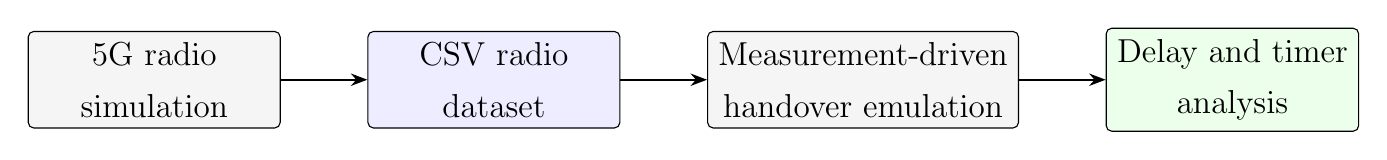
\begin{tikzpicture}[
  node distance=1.5cm and 1.1cm,
  stage/.style={draw, rounded corners=2pt, minimum width=3.2cm, minimum height=0.9cm, align=center, fill=gray!8},
  data/.style={draw, rounded corners=2pt, minimum width=3.2cm, minimum height=0.9cm, align=center, fill=blue!7},
  result/.style={draw, rounded corners=2pt, minimum width=3.2cm, minimum height=0.9cm, align=center, fill=green!8},
  flow/.style={-{Stealth[scale=0.9]}, thick}
]
\node[stage] (sim) {5G radio\\simulation};
\node[data, right=of sim] (csv) {CSV radio\\dataset};
\node[stage, right=of csv] (emu) {Measurement-driven\\handover emulation};
\node[result, right=of emu] (analysis) {Delay and timer\\analysis};

\draw[flow] (sim) -- (csv);
\draw[flow] (csv) -- (emu);
\draw[flow] (emu) -- (analysis);
\end{tikzpicture}
}
\caption{Overall workflow of radio-data generation and handover-delay analysis}
\label{fig:introduction-workflow}
\end{figure}

\subsection{Objectives}

The objective of this thesis is to build and evaluate a reproducible workflow for studying 5G radio measurements and handover delay. The work is designed around two connected parts. The first part focuses on generating radio-measurement data in a controlled simulation environment. The second part focuses on using measurement-driven handover experiments and logs to analyze the delay of the handover procedure. By combining these two parts, the thesis aims to provide a clearer view of how radio conditions motivate mobility decisions and how protocol execution determines the final handover completion behavior.

From a functional perspective, the workflow should be able to simulate UE movement, calculate relevant radio parameters, select or record serving-cell behavior, and export the generated measurements into a structured CSV format. It should also support handover-delay experiments in which timer events and network-condition effects can be inspected. These functional requirements are important because the output of the system must be directly usable for later analysis, instead of only producing visual observations or final summary values.

From a non-functional perspective, the workflow should be reproducible, configurable, and suitable for repeated experiments. Reproducibility is important because the same scenario should be rerun and verified under controlled settings. Configurability is needed because different UE heights, movement paths, radio conditions, and network-delay settings may be examined. The output format should also be clear enough to support post-processing, comparison, and visualization without requiring manual interpretation of unstructured logs.

The specific objectives are:

\begin{itemize}
    \item generate structured radio-measurement data from a controllable 5G propagation simulation;
    \item record key mobility and radio parameters, including UE position, serving cell, RSRP, SINR, and handover indicators;
    \item use measurement-driven handover experiments to observe protocol-level handover behavior;
    \item analyze how timer behavior and network conditions affect handover completion time, timeout cases, and failure behavior.
\end{itemize}

\subsection{Scope}

The thesis focuses on simulation-based radio-data generation and log-based handover-delay analysis. The radio-data generation part is limited to the implemented 5G propagation and mobility simulation workflow. It considers the parameters that are available in the simulator, such as UE position, gNB position, propagation-related values, serving-cell information, RSRP, SINR, and handover-related indicators. The purpose of this part is not to reproduce every detail of a commercial 5G network, but to create a controlled and explainable dataset that can be used to inspect mobility behavior under selected scenarios.

The handover-delay analysis part is limited to the implemented measurement-driven handover-emulation workflow and the available experiment logs. The analysis focuses on completion time, timeout behavior, failure cases, and the influence of network conditions such as latency, packet loss, and jitter. It does not attempt to model every internal mechanism of a full 5G core deployment or every vendor-specific handover implementation. Instead, it uses the available timer and event logs to study how protocol-level execution contributes to the observed handover delay.

This thesis does not attempt to perform a full real-world 5G measurement campaign. Such a campaign would require specialized equipment, controlled field conditions, repeated physical measurements, and access to operational network configurations. The thesis also does not aim to design a complete commercial handover optimization algorithm. Although the generated data and delay analysis can support future optimization work, the main focus here is on building the workflow, generating structured data, and analyzing the resulting handover delay characteristics.

\subsection{Main Contributions}

The main contributions of this thesis are:

\begin{itemize}
    \item a reproducible workflow for generating 5G radio-measurement datasets;
    \item a structured CSV output format for mobility and handover-related analysis;
    \item an analysis of handover delay and timer behavior under selected network conditions.
\end{itemize}

The first contribution is the construction of a reproducible radio-data generation workflow. Instead of relying only on manually collected or incomplete measurement data, the workflow allows selected mobility scenarios to be simulated and recorded in a consistent manner. This makes it possible to inspect how the radio environment changes along a UE trajectory and how those changes are reflected in the generated measurements.

The second contribution is the structured CSV output format. By recording relevant fields such as UE position, serving cell, radio measurements, and handover indicators, the dataset can be used for later processing and comparison. A structured format also reduces ambiguity because each recorded value has a clear role in the analysis pipeline. This is useful for both direct inspection and future extensions, such as visualization, statistical analysis, or machine-learning-based studies.

The third contribution is the analysis of handover delay and timer behavior under selected network conditions. The thesis examines how delay, timeout cases, failure behavior, and recovery margin can be affected by protocol timers and network impairments. This provides a more detailed view of handover performance than a simple success-or-failure summary.

\subsection{Thesis Organization}

The remainder of this thesis is organized as follows:

\noindent\hspace*{1cm}Chapter 2. Theoretical Background\\
\hspace*{1cm}Chapter 3. System Design\\
\hspace*{1cm}Chapter 4. Experimental Results\\
\hspace*{1cm}Chapter 5. Conclusion

\pagebreak 
 
\section*{CHAPTER 2. CELLULAR NETWORK AND MOBILITY MANAGEMENT}
\addcontentsline{toc}{section}{\protect\numberline{}CHAPTER 2. CELLULAR NETWORK AND MOBILITY MANAGEMENT}
\setcounter{section}{2}
\setcounter{subsection}{0}
\setcounter{figure}{0}
\setcounter{table}{0}
\subsection{Overview of 5G Network Architecture and A2G Communication}

The 5G mobile network is designed to support three main service objectives: Enhanced Mobile Broadband (eMBB) for high data rate services, Ultra-Reliable Low Latency Communications (URLLC) for delay-sensitive and reliable services, and Massive Machine-Type Communications (mMTC) for connecting a large number of devices \cite{itu_m2083}. In a basic 5G system, the UE is the terminal device that accesses the mobile network. A UE can be a smartphone, an Internet of Things (IoT) device, or in an aerial communication scenario, an unmanned aerial vehicle (UAV) acting as an aerial UE.

The UE connects to the radio access network (RAN) through a base station (BS), referred to in 5G as a gNB. The gNB is responsible for providing the wireless radio interface, transmitting and receiving radio signals, managing radio resources, and maintaining the radio connection with the UE. It also forwards user data and control information between the UE and the 5G Core (5GC) network. Therefore, the gNB is the main network element that directly determines how the UE accesses the 5G system over the air interface.

In a conventional terrestrial scenario, the UE is usually located near the ground and moves inside the coverage area of surrounding gNBs. The radio link quality is mainly affected by the horizontal distance between the UE and the serving gNB, obstacles such as buildings or terrain, shadow fading, and interference from neighboring cells.

Air-to-ground (A2G) communication extends this model by considering a UAV or aerial UE communicating with ground-based gNBs. This corresponds to the cellular-connected UAV case, where the UAV acts as a flying mobile terminal within a cellular network \cite{mozaffari2019tutorial,zeng2019accessing}. Unlike a ground UE, an aerial UE operates at a certain altitude and can have LOS or near-LOS paths to several BSs. This difference changes the radio propagation condition because the signal quality is affected not only by horizontal distance, but also by altitude, three-dimensional distance, and the elevation angle between the UAV and each gNB \cite{zeng2016uav}.

As the UAV moves, these geometric factors can change continuously. A higher altitude may improve visibility to the serving gNB, but it may also expose the UAV to stronger interference from multiple neighboring gNBs; this LoS-dominant channel and aerial-terrestrial interference are highlighted as key issues for UAV communications in 5G and beyond \cite{zeng2019accessing}. For this reason, important radio measurements such as RSRP and SINR may vary rapidly in A2G scenarios. These variations make A2G communication an important case for studying radio measurement behavior and mobility-related problems in 5G networks.

\begin{figure}[H]
\centering
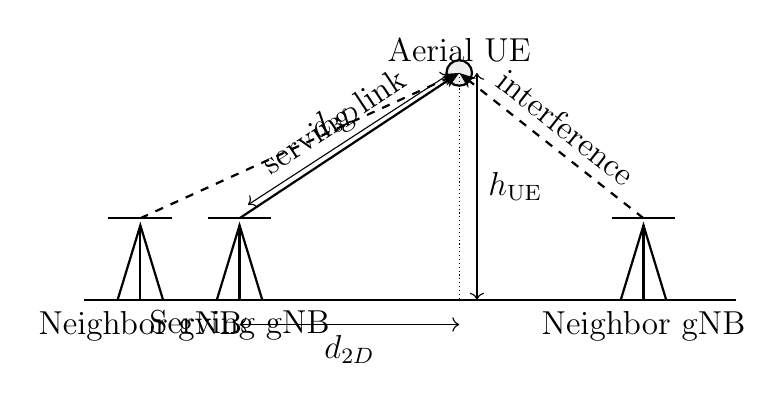
\begin{tikzpicture}[scale=0.9, every node/.style={font=\small}]
    \draw[thick] (-1.2,0) -- (8.0,0);

    \coordinate (serving) at (1.0,1.15);
    \coordinate (ue) at (4.1,3.2);
    \coordinate (ueproj) at (4.1,0);
    \coordinate (intone) at (6.7,1.15);
    \coordinate (inttwo) at (-0.4,1.15);

    \foreach \x/\name in {1.0/Serving gNB,6.7/Neighbor gNB,-0.4/Neighbor gNB}{
        \draw[thick] (\x,0) -- (\x,1.05);
        \draw[thick] (\x-0.32,0) -- (\x,1.05) -- (\x+0.32,0);
        \draw[thick] (\x-0.45,1.15) -- (\x+0.45,1.15);
        \node[below] at (\x,0) {\name};
    }

    \draw[fill=gray!15, thick] (ue) circle (0.18);
    \node[above] at (ue) {Aerial UE};
    \draw[densely dotted] (ue) -- (ueproj);

    \draw[arrow] (serving) -- node[above, sloped] {serving link} (ue);
    \draw[arrow, dashed] (intone) -- node[above, sloped] {interference} (ue);
    \draw[arrow, dashed] (inttwo) -- (ue);

    \draw[<->] (1.0,-0.35) -- node[below] {\(d_{2D}\)} (4.1,-0.35);
    \draw[<->] (4.35,0) -- node[right] {\(h_{\mathrm{UE}}\)} (4.35,3.2);
    \draw[<->] (1.12,1.34) -- node[above, sloped] {\(d_{3D}\)} (3.95,3.18);
\end{tikzpicture}
\caption{A2G radio scenario with serving-gNB connection, neighboring-gNB interference, and geometry-dependent link measurements}
\label{fig:a2g-radio-scenario}
\end{figure}

\subsection{Cellular Network and Mobility Models}

The spatial arrangement of gNBs and the movement pattern of UEs are important factors in cellular network analysis. The network layout determines the relative positions of serving and neighboring gNBs, while the mobility model determines how the UE position changes over time. These two elements directly influence propagation distance, received signal strength, interference, and mobility-related events. This thesis considers a hexagonal cellular layout and the Manhattan mobility model as the theoretical basis for representing the network geometry and UE movement.

\subsubsection{Hexagonal Cellular Network Model}

The hexagonal cellular model is a conceptual approximation used to represent the radio coverage of a BS. In an ideal isotropic environment, equal received-power contours around a BS would be approximately circular. Actual cell boundaries, however, are irregular because they are shaped by terrain, buildings, antenna patterns, propagation loss, and interference. Therefore, a hexagonal cell should not be interpreted as the exact physical coverage boundary of a gNB, but as a simplified geometric abstraction for network planning and analysis \cite{rappaport2002}.

Circular cells cannot cover a large two-dimensional area without leaving gaps or creating overlaps. Regular hexagons, in contrast, tessellate the plane exactly and approximate circular coverage more closely than the other regular polygons that can tessellate the plane \cite{rappaport2002}. The hexagonal representation consequently provides both a simple approximation of radio coverage and a consistent structure for placing neighboring gNBs. Each cell has six immediate neighbors, which facilitates the analysis of inter-cell interference, cell association, and handover (HO) behavior.

\begin{figure}[H]
\centering
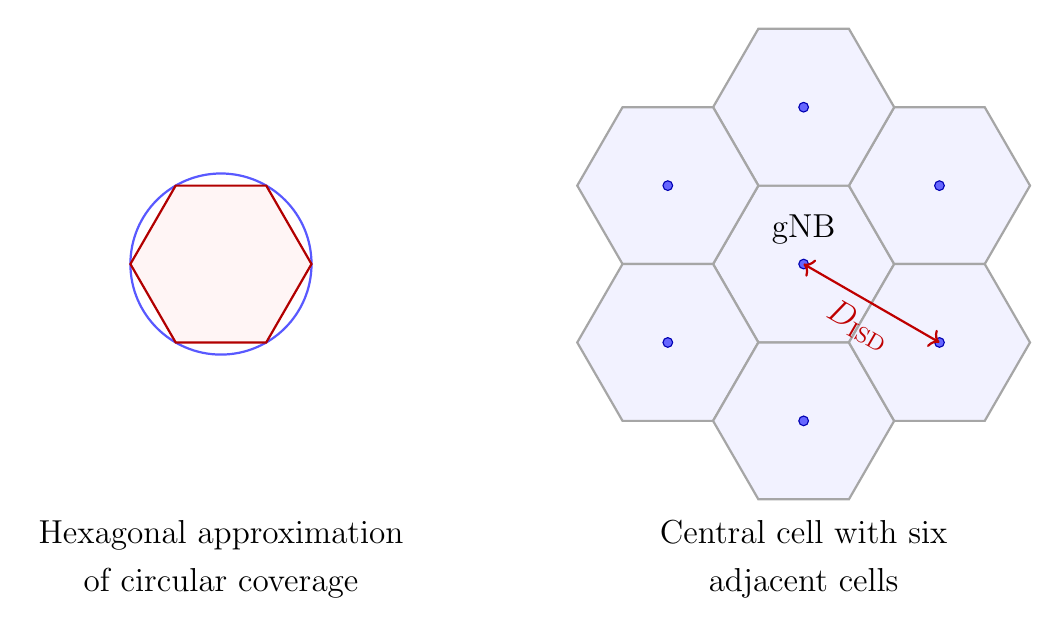
\begin{tikzpicture}[
    station/.style={
        circle,
        draw=blue!70!black,
        fill=blue!60,
        minimum size=3.5pt,
        inner sep=0pt
    }
]
\def\hexradius{1.15}

% Circular coverage approximation
\draw[blue!65, thick] (-3.8,0) circle[radius=\hexradius cm];
\draw[red!70!black, thick, fill=red!4]
    ({-3.8+\hexradius*cos(0)},   {\hexradius*sin(0)})
    \foreach \angle in {60,120,...,300} {
        -- ({-3.8+\hexradius*cos(\angle)}, {\hexradius*sin(\angle)})
    } -- cycle;
\node[align=center, font=\small] at (-3.8,-3.75)
    {Hexagonal approximation\\of circular coverage};

% Seven-cell hexagonal layout
\foreach \cx/\cy in {
    3.6/0,
    5.325/0.99593,
    3.6/1.99186,
    1.875/0.99593,
    1.875/-0.99593,
    3.6/-1.99186,
    5.325/-0.99593
}{
    \draw[gray!70, thick, fill=blue!5]
        ({\cx+\hexradius*cos(0)}, {\cy+\hexradius*sin(0)})
        \foreach \angle in {60,120,...,300} {
            -- ({\cx+\hexradius*cos(\angle)}, {\cy+\hexradius*sin(\angle)})
    } -- cycle;
    \node[station] at (\cx,\cy) {};
}
\draw[<->, thick, red!75!black] (3.6,0) -- node[below, sloped, font=\small] {$D_{\mathrm{ISD}}$} (5.325,-0.99593);
\node[above=3pt, font=\small] at (3.6,0) {gNB};
\node[align=center, font=\small] at (3.6,-3.75)
    {Central cell with six\\adjacent cells};
\end{tikzpicture}
\caption{Circular coverage approximation and seven-cell hexagonal layout}
\label{fig:hexagonal-cellular-layout}
\end{figure}

The distance between the centers of two adjacent cells is commonly referred to as the inter-site distance (ISD). For a regular hexagonal cell with radius \(R\), measured from the center to a vertex, the ISD is

\begin{equation}
    D_{\mathrm{ISD}} = \sqrt{3}R.
\end{equation}

The cell radius and ISD determine the spatial density of gNB deployment. A smaller ISD produces a denser network, which may improve coverage but also increases the possibility of inter-cell interference. Conversely, a larger ISD reduces the number of gNBs in a given area but may result in weaker received power near cell boundaries. Therefore, the hexagonal model is useful for studying coverage, neighboring-cell interference, cell association, and HO behavior.

\subsubsection{Manhattan Mobility Model}

The Manhattan mobility model is a geographic-restriction mobility model designed to represent movement on an urban street grid \cite{bai2003}. The service area is divided into horizontal and vertical road segments that form an orthogonal grid. A UE moves only along these road segments and may travel in one of four directions: North, South, East, or West. Direction changes are permitted at intersections, where the UE may continue forward or select another valid road while remaining inside the service area.

\begin{figure}[H]
\centering
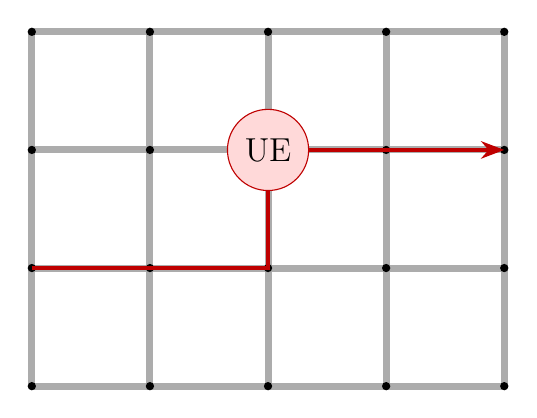
\begin{tikzpicture}[
    road/.style={gray!65, line width=2.5pt},
    route/.style={-{Stealth[scale=0.9]}, red!75!black, line width=1.4pt},
    intersection/.style={circle, fill=black, minimum size=3pt, inner sep=0pt}
]
\foreach \x in {0,1.5,3,4.5,6}
    \draw[road] (\x,0) -- (\x,4.5);
\foreach \y in {0,1.5,3,4.5}
    \draw[road] (0,\y) -- (6,\y);
\foreach \x in {0,1.5,3,4.5,6}
    \foreach \y in {0,1.5,3,4.5}
        \node[intersection] at (\x,\y) {};
\draw[route] (0,1.5) -- (3,1.5) -- (3,3) -- (6,3);
\node[circle, draw=red!75!black, fill=red!15, minimum size=7mm] at (3,3) {\small UE};
\end{tikzpicture}
\caption{Example of UE movement in a Manhattan street grid}
\label{fig:manhattan-mobility}
\end{figure}

UE movement is considered continuous along each road segment. During one simulation interval, the travel distance is determined by the UE speed and the duration of the time step:

\begin{equation}
    d_{\mathrm{move}} = v \Delta t,
\end{equation}

where \(d_{\mathrm{move}}\) is the distance traveled during one time step, \(v\) is the UE speed, and \(\Delta t\) is the time-step duration. At an intersection, the movement direction may be updated according to the set of available directions. Additional behaviors such as temporary stops or gradual acceleration can also be included to represent traffic conditions, but they are not fundamental requirements of the Manhattan model.

The Manhattan model provides a more structured representation of urban mobility than unconstrained random movement. As the UE moves along the street grid, its distance and relative direction to surrounding gNBs change over time. These changes lead to variations in path loss, shadow fading, RSRP, and SINR, and may eventually cause the UE to change its serving gNB. Thus, the combination of the hexagonal network model and Manhattan mobility model provides a geometric foundation for studying radio measurements and HO behavior in a cellular network.

\subsection{Radio Propagation in 5G Networks and Measurement Metrics}

Radio propagation describes how the transmitted electromagnetic signal changes before it reaches the receiver. In a 5G cellular network, the received signal is affected by distance, carrier frequency, antenna gains, LOS or NLOS condition, shadowing objects, interference from other cells, and receiver noise. 3GPP TR 38.901 provides the commonly used channel-modelling framework for frequencies from 0.5 GHz to 100 GHz, including path loss, LOS probability, penetration loss, shadow fading, and fast-fading components for scenarios such as Urban Macro (UMa) and Urban Micro (UMi) \cite{3gpp_38901}. This thesis uses these concepts at a system-simulation level to generate interpretable radio measurements rather than to reproduce a full link-level channel realization.

For a UE and a gNB separated by horizontal distance \(d_{2D}\), the three-dimensional link distance is

\begin{equation}
    d_{3D} = \sqrt{d_{2D}^{2} + (h_{\mathrm{UE}} - h_{\mathrm{gNB}})^{2}},
\end{equation}

where \(h_{\mathrm{UE}}\) and \(h_{\mathrm{gNB}}\) are the UE and gNB antenna heights. This distance is especially important in A2G scenarios because a change in UE height changes both the link distance and the elevation geometry. A higher aerial UE may have a higher LOS probability to several gNBs, but the same visibility can also increase received interference from neighboring cells.

\subsubsection{Large-Scale Propagation Components Used in the Simulator}

The radio simulator uses a large-scale propagation abstraction rather than a full small-scale fading channel. This abstraction is appropriate for generating mobility traces because the quantities of interest are serving-cell strength, neighboring-cell strength, and SINR trends along the UE trajectory. The theoretical chain used in the simulator is

\begin{equation}
\{d_{2D},d_{3D},h_{\mathrm{UE}}\}
\rightarrow P_{\mathrm{LOS}}
\rightarrow S_{\mathrm{LOS/NLOS}}
\rightarrow PL
\rightarrow X_{\sigma}
\rightarrow \{P_{\mathrm{rx}},\mathrm{RSRP},\mathrm{SINR}\}.
\end{equation}

In this chain, geometry determines path length and LOS probability. The sampled LOS/NLOS state selects the path-loss formula. Shadow fading adds a spatially varying large-scale random term. Finally, the link budget and interference model convert these losses into received power, RSRP, and SINR.

\begin{table}[H]
\centering
\caption{Theoretical propagation components used by the radio simulator \cite{3gpp_38901,3gpp_36777,3gpp_38215}}
\small
\begin{tabularx}{\textwidth}{>{\raggedright\arraybackslash}p{3.0cm}>{\raggedright\arraybackslash}X>{\raggedright\arraybackslash}p{4.1cm}}
\toprule
Component & Theoretical role & Dataset quantity\\
\midrule
Link geometry & Defines horizontal distance, 3D distance, UE height, and the applicable terrestrial or aerial regime. & UE/gNB position, height, distance\\
LOS/NLOS condition & Represents the probability and realization of direct visibility between UE and gNB. & LOS probability, LOS state\\
Path loss & Models median large-scale attenuation due to distance, frequency, height, and propagation condition. & Path loss\\
Shadow fading & Models slow random variation around the median path loss caused by environmental obstruction. & Shadow-fading value\\
Link measurement & Converts propagation loss, antenna gains, noise, and interference into radio measurement indicators. & Received power, RSRP, SINR\\
\bottomrule
\end{tabularx}
\label{tab:theoretical-propagation-components}
\end{table}

\subsubsection{LOS Probability and LOS/NLOS State}

The simulator first calculates a LOS probability for each UE--gNB link. The model follows the UMa LOS probability in 3GPP TR 38.901 for terrestrial and low-height UEs and the UMa-AV extension in 3GPP TR 36.777 for aerial UEs \cite{3gpp_38901,3gpp_36777}. The NLOS probability is then

\begin{equation}
    P_{\mathrm{NLOS}} = 1 - P_{\mathrm{LOS}}.
\end{equation}

Here, \(\operatorname{clip}(x,0,1)\) denotes limiting \(x\) to the interval \([0,1]\). All distances in the following LOS-probability expressions are in metres.

The implemented LOS-probability calculation can be followed from the UE height range and then from the horizontal distance \(d_{2D}\). For terrestrial and low-height UEs, \(1.5 \le h_{\mathrm{UE}} \le 22.5\) m, the simulator uses the UMa expression from 3GPP TR 38.901 \cite{3gpp_38901}. If the UE is very close to the gNB in the horizontal plane, \(d_{2D}\le18\) m, the link is treated as LOS with

\begin{equation}
    P_{\mathrm{LOS}}=1.
\end{equation}

When \(d_{2D}>18\) m, the LOS probability decreases with distance but includes a height correction for UEs above 13 m:

\begin{align}
    P_{\mathrm{LOS}}
    &= \operatorname{clip}\left(P_{\mathrm{base}}G_h,0,1\right),\\
    P_{\mathrm{base}}
    &= \frac{18}{d_{2D}}+
       \left(1-\frac{18}{d_{2D}}\right)
       e^{-d_{2D}/63},\\
    G_h
    &= 1+\frac{5}{4}C(h_{\mathrm{UE}})
       \left(\frac{d_{2D}}{100}\right)^3
       e^{-d_{2D}/150}.
\end{align}

The height correction is inactive for ordinary ground-level UEs and becomes active only when \(h_{\mathrm{UE}}>13\) m:

\begin{equation}
C(h_{\mathrm{UE}})=
\begin{cases}
0, & h_{\mathrm{UE}}\le13,\\
\left(\dfrac{h_{\mathrm{UE}}-13}{10}\right)^{1.5},
& 13<h_{\mathrm{UE}}\le22.5.
\end{cases}
\end{equation}

For aerial UEs in the range \(22.5<h_{\mathrm{UE}}\le100\) m, the simulator switches to the UMa-AV LOS-probability model from 3GPP TR 36.777 \cite{3gpp_36777}. It first calculates two height-dependent parameters:

\begin{align}
    d_1 &= \max\left(460\log_{10}(h_{\mathrm{UE}})-700,18\right),\\
    p_1 &= 4300\log_{10}(h_{\mathrm{UE}})-3800.
\end{align}

The value \(d_1\) acts as the first horizontal-distance threshold. If \(d_{2D}\le d_1\), the link is treated as LOS:

\begin{equation}
    P_{\mathrm{LOS}}=1.
\end{equation}

If \(d_{2D}>d_1\), the LOS probability is reduced according to

\begin{equation}
    P_{\mathrm{LOS}}=
    \operatorname{clip}\left(
    \frac{d_1}{d_{2D}}+
    e^{-d_{2D}/p_1}
    \left(1-\frac{d_1}{d_{2D}}\right),
    0,1\right).
\end{equation}

Finally, for high aerial UEs, \(100<h_{\mathrm{UE}}\le300\) m, the implemented model sets

\begin{equation}
    P_{\mathrm{LOS}}=1.
\end{equation}

After \(P_{\mathrm{LOS}}\) is calculated, the simulator converts this probability into a concrete LOS/NLOS state by Bernoulli sampling. For each UE--gNB link, a uniform random variable \(u\sim\mathcal{U}(0,1)\) is drawn and the link state \(S\) is assigned as

\begin{equation}
S=
\begin{cases}
\mathrm{LOS}, & u \le P_{\mathrm{LOS}},\\
\mathrm{NLOS}, & u > P_{\mathrm{LOS}}.
\end{cases}
\end{equation}

Thus, a larger \(P_{\mathrm{LOS}}\) gives a higher chance that the link is realized as LOS, while \(P_{\mathrm{LOS}}=1\) always gives a LOS link and \(P_{\mathrm{LOS}}=0\) always gives a NLOS link. The sampled LOS/NLOS state is then cached once for each UE--gNB link and reused in the subsequent path-loss and shadow-fading calculations. This prevents the same link from randomly switching between LOS and NLOS at every time step and makes the generated trace easier to interpret.

\subsubsection{Path-Loss Model}

Path loss represents the large-scale attenuation between the transmitter and receiver. It increases with distance and depends on the propagation environment, carrier frequency, UE height, and LOS/NLOS state. The simulator follows the same order as the implementation in \texttt{radio\_models.py}: first it prepares effective distances, then it selects the UMa or UMa-AV formula according to UE height and sampled LOS/NLOS state. The low-height UMa formulas are based on 3GPP TR 38.901, and the aerial UMa-AV formulas are based on 3GPP TR 36.777 \cite{3gpp_38901,3gpp_36777}.

Before evaluating path loss, the horizontal distance is lower-bounded by 10 m and the effective 3D distance is recomputed:

\begin{align}
    d_{2D,\mathrm{eff}} &= \max(d_{2D},10),\\
    d_{3D,\mathrm{eff}} &=
    \sqrt{d_{2D,\mathrm{eff}}^2+
    (h_{\mathrm{gNB}}-h_{\mathrm{UE}})^2}.
\end{align}

For readability, the following path-loss equations use \(d_{2D}\) and \(d_{3D}\) to denote these effective distances after preprocessing.

The UMa LOS formula also uses the effective breakpoint distance

\begin{equation}
    d'_{\mathrm{BP}} =
    \frac{4(h_{\mathrm{gNB}}-1)(h_{\mathrm{UE}}-1)f_c}{c},
\end{equation}

where \(f_c\) is in Hz and \(c\) is the speed of light. In the remaining path-loss formulas, \(f_{c,\mathrm{GHz}}\) denotes the carrier frequency in GHz.

For \(1.5 \le h_{\mathrm{UE}} \le 22.5\) m, the simulator uses the UMa path-loss model. If the sampled link state is LOS and \(d_{2D}\le d'_{\mathrm{BP}}\), the LOS path loss is

\begin{equation}
    PL_{\mathrm{LOS}} =
    28+22\log_{10}(d_{3D})
    +20\log_{10}(f_{c,\mathrm{GHz}}).
\end{equation}

If the same low-height LOS link is beyond the breakpoint, \(d_{2D}>d'_{\mathrm{BP}}\), the slope changes to

\begin{align}
    PL_{\mathrm{LOS}} &=
    28+40\log_{10}(d_{3D})
    +20\log_{10}(f_{c,\mathrm{GHz}}) \nonumber\\
    &\quad -9\log_{10}\left(
    (d'_{\mathrm{BP}})^2+
    (h_{\mathrm{gNB}}-h_{\mathrm{UE}})^2
    \right).
\end{align}

If the sampled low-height link state is NLOS, the simulator first computes

\begin{align}
    PL'_{\mathrm{NLOS}} &=
    13.54+39.08\log_{10}(d_{3D})
    +20\log_{10}(f_{c,\mathrm{GHz}}) \nonumber\\
    &\quad -0.6(h_{\mathrm{UE}}-1.5),
\end{align}

and then applies the 3GPP max operation:

\begin{equation}
    PL_{\mathrm{NLOS}} =
    \max\left(PL_{\mathrm{LOS}},PL'_{\mathrm{NLOS}}\right).
\end{equation}

For aerial UEs, \(22.5<h_{\mathrm{UE}}\le300\) m, the LOS path-loss expression becomes the UMa-AV LOS formula:

\begin{equation}
    PL_{\mathrm{LOS,AV}} =
    28+22\log_{10}(d_{3D})
    +20\log_{10}(f_{c,\mathrm{GHz}}).
\end{equation}

For aerial NLOS links, the implemented UMa-AV NLOS expression is defined for \(22.5<h_{\mathrm{UE}}\le100\) m:

\begin{align}
    PL_{\mathrm{NLOS,AV}} &=
    -17.5+
    \left(46-7\log_{10}(h_{\mathrm{UE}})\right)
    \log_{10}(d_{3D}) \nonumber\\
    &\quad +20\log_{10}\left(
    \frac{40\pi f_{c,\mathrm{GHz}}}{3}
    \right).
\end{align}

The path loss stored in the dataset is selected according to the cached LOS/NLOS state:

\begin{equation}
PL =
\begin{cases}
PL_{\mathrm{LOS}}, & \text{for a low-height LOS link},\\
PL_{\mathrm{NLOS}}, & \text{for a low-height NLOS link},\\
PL_{\mathrm{LOS,AV}}, & \text{for an aerial LOS link},\\
PL_{\mathrm{NLOS,AV}}, & \text{for an aerial NLOS link with } 22.5<h_{\mathrm{UE}}\le100.
\end{cases}
\end{equation}

Thus, the logged path-loss value is not only a function of distance. It also reflects UE height, LOS probability, sampled LOS/NLOS state, carrier frequency, and the UMa or UMa-AV scenario selected for the link.

\subsubsection{Shadow-Fading Model}

Shadow fading models slower received-power variation caused by obstacles and local environmental structure that are not captured by distance-only path loss. It is commonly represented as a log-normal random component, or equivalently as a Gaussian random variable in dB. In the implemented simulator, the shadow-fading loss for a UE--gNB link is sampled as

\begin{equation}
    X_{\sigma}\sim\mathcal{N}(0,\sigma_{\mathrm{SF}}^2),
\end{equation}

where \(\sigma_{\mathrm{SF}}\) is selected from the corresponding LOS/NLOS and UE-height condition. For UMa-AV links, the standard deviation follows the shadow-fading parameters in 3GPP TR 36.777 Annex B, with the low-height UMa values referenced from TR 38.901 \cite{3gpp_36777,3gpp_38901}. The simulator uses

\begin{equation}
\sigma_{\mathrm{SF}} =
\begin{cases}
4~\mathrm{dB}, & 1.5\le h_{\mathrm{UE}}\le22.5~\mathrm{m},~\mathrm{LOS},\\
6~\mathrm{dB}, & 1.5\le h_{\mathrm{UE}}\le22.5~\mathrm{m},~\mathrm{NLOS},\\
4.64e^{-0.0066h_{\mathrm{UE}}}~\mathrm{dB}, & 22.5<h_{\mathrm{UE}}\le300~\mathrm{m},~\mathrm{LOS},\\
6~\mathrm{dB}, & 22.5<h_{\mathrm{UE}}\le100~\mathrm{m},~\mathrm{NLOS}.
\end{cases}
\end{equation}

For the default ground-UE mode, the implementation can also use fixed configured values, \(\sigma_{\mathrm{SF}}=4.6\) dB for LOS and \(10\) dB for NLOS, as defined in \texttt{config.py}. This separates the baseline terrestrial configuration from the UMa-AV height-dependent configuration used for aerial-UE studies.

The sampled value is clipped to the interval \([-3\sigma_{\mathrm{SF}},3\sigma_{\mathrm{SF}}]\). This clipping avoids unrealistically large random losses in finite simulation traces while preserving the zero-mean Gaussian behaviour for most samples. The received power including shadow fading is then

\begin{equation}
    P_{\mathrm{rx}} = P_{\mathrm{tx}} + G_{\mathrm{tx}} + G_{\mathrm{rx}} - PL - X_{\sigma},
\end{equation}

where \(P_{\mathrm{tx}}\) is the transmit power, \(G_{\mathrm{tx}}\) and \(G_{\mathrm{rx}}\) are antenna gains, \(PL\) is path loss, and \(X_{\sigma}\) is the shadow-fading term. A positive shadow-fading realization reduces the received power, while a negative realization improves it relative to the median path-loss value. This explains why two UE positions with similar distance to the serving gNB may still produce different received powers.

The simulator does not resample shadow fading independently at every time step. Instead, the current shadow-fading value is cached for each UE--gNB link and reused while the accumulated UE movement for that link remains below 25 m. Once the accumulated movement reaches 25 m, a new \(X_{\sigma}\) value is sampled and the accumulated distance is reset. This 25 m update distance implements a simple spatial-consistency approximation for large-scale fading, following the distance-dependent shadowing treatment used in 3GPP channel modelling \cite{3gpp_36777}. As a result, shadow fading changes more slowly than instantaneous RSRP or SINR calculations and avoids artificial step-to-step randomness in the generated measurement trace.

Reference Signal Received Power (RSRP) is a key measurement for assessing cell strength. In NR, 3GPP TS 38.215 defines SS-RSRP and CSI-RSRP as linear averages of the power contributions of resource elements carrying the corresponding synchronization-signal or CSI reference signals \cite{3gpp_38215}. In this thesis, RSRP is used as a system-level approximation of reference-signal power derived from the received downlink power. It provides a compact indicator of serving-cell and neighboring-cell strength and is therefore useful for comparing candidate gNBs along a UE trajectory.

Interference is produced by transmissions from non-serving cells that reuse the same time-frequency resources or overlap with the measured resources. Unlike thermal noise, interference depends on the topology, the UE position, the serving gNB, and the received powers from surrounding gNBs. A UE near a cell edge, or an aerial UE with LOS visibility to several gNBs, may observe strong desired-signal power and strong interference at the same time. For this reason, RSRP alone is not sufficient to describe link quality.

Receiver noise is commonly modelled from the thermal noise density and receiver noise figure:

\begin{equation}
    N_{\mathrm{dBm}} = -174 + 10\log_{10}(B) + NF,
\end{equation}

where \(B\) is the receiver bandwidth in Hz and \(NF\) is the receiver noise figure in dB. The value \(-174\) dBm/Hz is the approximate thermal noise power spectral density at room temperature \cite{rappaport2002}. Noise is independent of the serving-cell choice, but it becomes important when the received signal and interference powers are low.

Signal-to-Interference-plus-Noise Ratio (SINR) combines the desired signal, interference, and noise into one quality metric. In linear scale, it is written as

\begin{equation}
    \mathrm{SINR} = \frac{P_{\mathrm{serving}}}{\sum_{i=1}^{N_{\mathrm{int}}} P_{\mathrm{int},i} + P_{\mathrm{noise}}},
\end{equation}

and in dB as

\begin{equation}
    \mathrm{SINR}_{\mathrm{dB}} = 10\log_{10}(\mathrm{SINR}).
\end{equation}

3GPP TS 38.215 also specifies NR physical-layer SINR measurements, including SS-SINR and CSI-SINR, based on reference-signal resources and corresponding interference-plus-noise contributions \cite{3gpp_38215}. Conceptually, SINR is more directly related to link quality than RSRP because it penalizes both weak serving-signal power and strong interference. Thus, a UE can have acceptable RSRP but poor SINR if neighboring cells are received strongly.

The radio-measurement dataset generated in this thesis records these propagation and measurement concepts in structured form. UE position, height, velocity, and direction describe the mobility state. Serving-cell information identifies the current associated gNB. LOS probability and LOS state describe the propagation condition. Path loss, shadow fading, received power, RSRP, neighboring-cell RSRP, and SINR describe the radio environment observed by the UE at each simulation step. Together, these fields make it possible to inspect how movement changes radio conditions and how those changes may affect cell association and handover-related behavior.

\subsection{Handover in 5G Networks and Handover Delay}

???
định nghĩa. ví dụ: Handover delay is the time interval required for a UE to complete the transition from the source gNB to the target gNB.

\subsection{Chapter Conclusion}
This chapter presented the theoretical background related to 5G networks, A2G communication, radio propagation, radio measurement metrics, and handover delay. These concepts provide the foundation for the system design described in the next chapter.


\pagebreak

\section*{CHAPTER 3. INVESTIGATION OF MOBILITY MANAGEMENT IN AERIAL-TO-GROUND COMMUNICATIONS}
\addcontentsline{toc}{section}{\protect\numberline{}CHAPTER 3. INVESTIGATION OF MOBILITY MANAGEMENT IN AERIAL-TO-GROUND COMMUNICATIONS}
\setcounter{section}{3}
\setcounter{subsection}{0}
\setcounter{figure}{0}
\setcounter{table}{0}
\subsection{System Architecture}

The platform has two independently executable subsystems:

\begin{equation}
\text{Radio scenario}\rightarrow\text{measurement CSV}\rightarrow
\text{StormSim handover}\rightarrow\text{timer and delay results}.
\end{equation}

The first subsystem is the Python radio simulator. It generates mobility and radio measurements, including UE position, serving-cell selection, neighbor-cell RSRP, path loss, shadow fading, received power, and SINR. This subsystem is responsible for the radio-level view of the problem: it explains when the radio condition suggests that another gNB should become the serving cell.

The second subsystem is the protocol-level handover test environment. It uses a free5GC-based 5G Core and a Go-based UE--gNB emulator named StormSim in the implementation. free5GC provides the core-network side of the experiment, including AMF connectivity for NGAP/N2 signaling and user-plane support through GTP-U/N3 \cite{free5gc_project}. StormSim emulates the UE and gNB behavior required by the selected handover scenarios. It connects to the 5G Core, creates UE/gNB contexts, triggers Xn or N2 handover procedures, applies configurable transport impairment such as latency, packet loss, and jitter, and records trial-summary and timer-event logs.

The Python simulator and StormSim therefore have different responsibilities. The Python simulator does not execute the full handover signaling procedure, while StormSim does not replace the radio-propagation simulator. Instead, StormSim is used to study protocol-level execution after a target-cell transition is selected or replayed. Their current CSV schemas are not identical: the first exports \texttt{ue0\_connected\_bs}, while measurement mode expects \texttt{connected\_gnb} and \texttt{gnbX\_rsrp}.

\textbf{TODO: cần xác nhận từ người dùng.} Confirm the official schema-conversion step and input CSV.

\subsection{Radio Simulation Design}

\subsubsection{Network and Mobility}

The radio simulation subsystem is designed to generate structured radio-measurement traces from a controllable geometric scenario. The simulation area entered by the user is represented as a rectangular study region placed at the center of a 10 km by 10 km canvas. This separation between the full canvas and the active study rectangle makes it possible to draw the cellular layout around the region while keeping the UE movement bounded inside the selected area.

Ground gNBs are deployed on a flat-top hexagonal grid. The geometric hexagon radius is \(R=500\) m, so the distance between adjacent gNB centers is approximately \(\sqrt{3}R\), or about 866 m. This value is not entered manually for every gNB. Instead, the simulator generates enough candidate hexagonal sites to cover the user-defined rectangle and a surrounding buffer. As a result, the number of gNBs automatically follows the size of the selected study area.

UEs move on a Manhattan-style road grid inside the rectangular region. Each UE is initialized at a random road intersection and is assigned a valid cardinal direction. Within one simulation run, all UEs use the scenario UE height, while each UE receives an independent speed sample from the height-dependent speed range associated with that height. At each one-second simulation step, the basic movement distance is

\begin{equation}
    d_{\mathrm{move}}=v\Delta t,
\end{equation}

where \(v\) is the UE speed and \(\Delta t=1\) s. The movement model also includes a stop-and-go behavior: after a configured number of direction changes, the UE pauses for several steps and then gradually returns to its base speed. The detailed mobility behavior is described separately in Section~\ref{sec:ue-mobility-model}; this subsection focuses on how the mobility state is integrated into the radio-simulation workflow.

The gNB placement procedure follows the axial-coordinate representation for hexagonal grids. Each hexagon is stored as \((q,r)\), and the third cube coordinate is recovered as

\begin{equation}
    s=-q-r.
\end{equation}

This keeps the cube-coordinate constraint \(q+r+s=0\) while storing only two coordinates, which is a standard practical approach for hexagonal-grid algorithms \cite{redblob_hexagons}. The flat-top axial-to-Cartesian conversion used for the gNB layout is

\begin{align}
    x &= R\left(\frac{3}{2}q\right),\\
    y &= R\left(\sqrt{3}r+\frac{\sqrt{3}}{2}q\right),
\end{align}

where \(R\) is the geometric hexagon radius. These coordinates are shifted by the canvas center so that the generated grid is centered on the simulation map.

To adapt the topology to an arbitrary user-defined rectangle, the algorithm first estimates the axial coordinate ranges needed to cover the requested width and height:

\begin{align}
    q &\in \left[
    \mathrm{int}\left(-\frac{W}{1.5R}\right)-1,\,
    \mathrm{int}\left(\frac{W}{1.5R}\right)+1
    \right],\\
    r &\in \left[
    \mathrm{int}\left(-\frac{H}{\sqrt{3}R}\right)-1,\,
    \mathrm{int}\left(\frac{H}{\sqrt{3}R}\right)+1
    \right],
\end{align}

where \(W\) and \(H\) are the user-entered simulation width and height, and \(\mathrm{int}(\cdot)\) denotes integer conversion. The additional margin of one axial step avoids missing edge cells after the skewed axial grid is converted into Cartesian coordinates. The simulator then enumerates all \((q,r)\) pairs in these ranges, computes \(s=-q-r\), converts the hex center to Cartesian coordinates, and keeps only the centers that fall inside the simulation rectangle expanded by a boundary buffer:

\begin{equation}
    b=\frac{\sqrt{3}}{2}R.
\end{equation}

Thus a candidate gNB is retained when

\begin{equation}
    x_{\min}-b \le x \le x_{\max}+b,
    \qquad
    y_{\min}-b \le y \le y_{\max}+b.
\end{equation}

This design makes the gNB count a consequence of the requested study area instead of a fixed scenario constant. A larger rectangle automatically produces more hexagonal sites, while a smaller rectangle keeps only the sites needed near that region. The buffer also ensures that UEs near the simulation boundary still observe nearby external cells, reducing artificial edge effects in RSRP, SINR, and serving-cell selection.

\subsubsection{Radio Parameters}

\begin{table}[H]
\centering
\caption[Principal radio parameters]{Principal radio parameters \cite{3gpp_38901,3gpp_36777,3gpp_36104,3gpp_36101}}
\begin{tabular}{ll}
\toprule
Parameter & Value\\
\midrule
Carrier frequency & 2 GHz\\
gNB power & 46 dBm\\
gNB / UE antenna gain & 2 / 0 dB\\
Bandwidth / noise figure & 10 MHz / 9 dB\\
gNB / default UE height & 25 / 1.5 m\\
UE height range & 1.5--300 m\\
Handover margin & 3 dB\\
\bottomrule
\end{tabular}
\label{tab:principal-radio-parameters}
\end{table}

The table combines standardized propagation assumptions with implementation-level simulation settings used in the radio simulator. These values define the link budget, thermal-noise calculation, UE-height range, and RSRP-based serving-cell decision. The RSRP approximation used later assumes \(50\) LTE resource blocks for a 10 MHz carrier and \(12\) subcarriers per resource block; it is therefore a system-level approximation rather than an exact physical-layer CRS, SS-RSRP, or CSI-RSRP realization.

\subsubsection{Propagation-Model Calculation Flow}

The propagation model is executed for each UE--gNB candidate link at every simulation step. Its role is to transform the current geometry and UE height into radio fields that are later used for serving-cell selection, interference calculation, SINR calculation, and dataset generation. The model follows the theoretical chain introduced in Chapter 2, but here the focus is on how the chain is organized inside the simulator workflow.

The simulator does not rely on a separate terrestrial-versus-aerial mode switch. Instead, the UE height is the controlling input for the propagation regime. A low-height UE naturally falls into the UMa height range, while elevated UEs are evaluated by the UMa-AV expressions when their height enters the aerial range. This design keeps the radio calculation consistent across all altitude cases: the same processing chain is used, and only the height-dependent model selection changes.

\begin{figure}[H]
\centering
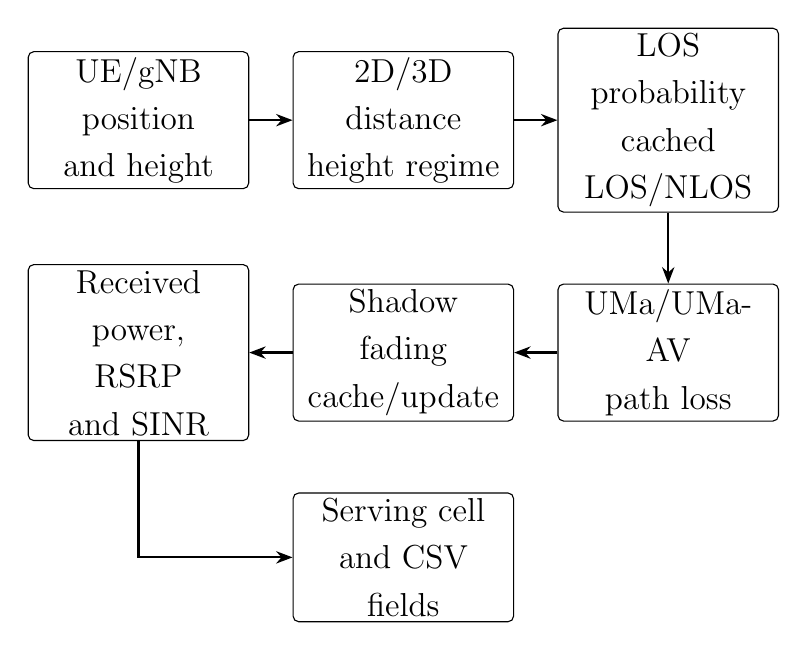
\begin{tikzpicture}[node distance=0.9cm and 0.55cm, font=\small]
    \node[box, text width=2.45cm] (geom) {UE/gNB\\position and height};
    \node[box, text width=2.45cm, right=of geom] (dist) {2D/3D distance\\height regime};
    \node[box, text width=2.45cm, right=of dist] (los) {LOS probability\\cached LOS/NLOS};
    \node[box, text width=2.45cm, below=of los] (pl) {UMa/UMa-AV\\path loss};
    \node[box, text width=2.45cm, left=of pl] (sf) {Shadow fading\\cache/update};
    \node[box, text width=2.45cm, left=of sf] (meas) {Received power,\\RSRP and SINR};
    \node[box, text width=2.45cm, below=of sf] (out) {Serving cell\\and CSV fields};

    \draw[arrow] (geom) -- (dist);
    \draw[arrow] (dist) -- (los);
    \draw[arrow] (los) -- (pl);
    \draw[arrow] (pl) -- (sf);
    \draw[arrow] (sf) -- (meas);
    \draw[arrow] (meas) |- (out);
\end{tikzpicture}
\caption{Propagation-model calculation flow in the radio simulator}
\label{fig:propagation-calculation-flow}
\end{figure}

\begin{table}[H]
\centering
\caption{Mapping of propagation-model calculations to simulator outputs}
\small
\begin{tabularx}{\textwidth}{>{\raggedright\arraybackslash}p{2.8cm}>{\raggedright\arraybackslash}X>{\raggedright\arraybackslash}p{4.0cm}}
\toprule
Stage & Operation in the simulator & Output used later\\
\midrule
Geometry & Use UE/gNB positions and heights to compute 2D/3D distances and select the low-height UMa or UMa-AV height regime. & Link distance and height regime\\
LOS state & Evaluate the LOS probability, then sample or reuse the cached Bernoulli LOS/NLOS state for each UE--gNB link. & \texttt{los\_probability}, \texttt{los\_state}\\
Path loss & Apply the UMa or UMa-AV formula according to distance, height, carrier frequency, and LOS/NLOS state. & \texttt{pathloss}\\
Shadow fading & Draw clipped Gaussian shadow fading, keep it in the link cache, and refresh it after 25 m of accumulated UE movement. & \texttt{shadow\_fading}\\
RSRP and SINR & Apply the link budget, map total received power to RSRP, add first-tier interference and thermal noise, and compute SINR. & RSRP, SINR, and neighbor-cell RSRP fields\\
\bottomrule
\end{tabularx}
\label{tab:propagation-implementation-mapping}
\end{table}

This flow is applied to candidate serving cells and to the first-tier interfering cells used in the SINR calculation. For each UE--gNB link, the sampled LOS/NLOS state and the current shadow-fading value are stored in a per-link cache. The shadow-fading value is reused while the UE movement accumulated for that link remains below 25 m, and a new value is sampled after the update distance is reached. This keeps the large-scale fading variation spatially smoother than an independently sampled value at every time step.

For a selected gNB, received power and RSRP are computed as

\begin{align}
P_{\mathrm{rx}} &= P_{\mathrm{tx}}+G_{\mathrm{tx}}+G_{\mathrm{rx}}-PL-SF,\\
\mathrm{RSRP} &= P_{\mathrm{rx}}-10\log_{10}(50\times12).
\end{align}

The SINR calculation uses the serving-link received power as the desired signal. Interference is calculated from the six nearest non-serving gNBs around the serving gNB, which approximate the first tier of co-channel interferers in the hexagonal layout. Thermal noise is then added to this interference term before converting the result to dB. This design makes SINR more sensitive than RSRP to aerial scenarios, because a higher UE can observe stronger received power from both the serving gNB and neighboring gNBs. The neighbor-cell RSRP fields are therefore not only auxiliary logging fields; they provide the radio context needed to explain why a UE may experience high serving-cell power while its SINR remains limited by interference.

\subsubsection{Handover Decision and Output}

The radio simulator uses an RSRP-based serving-cell rule. At initialization, the strongest candidate cell is selected as the serving gNB. After that, the current serving cell is kept unless a candidate cell exceeds the current serving-cell RSRP by the configured handover margin. Candidate \(c\) replaces serving cell \(s\) only when

\begin{equation}
\mathrm{RSRP}_{c}>\mathrm{RSRP}_{s}+3~\mathrm{dB}.
\end{equation}

There is no time-to-trigger, hysteresis timer, or SINR threshold in this radio-level serving-cell rule. Therefore, a recorded handover flag in the radio dataset should be interpreted as a serving-cell index transition suggested by the measurement model, not as a completed 5G protocol handover. This distinction is important because the radio simulator produces measurement traces and serving-cell events, while the protocol-level handover timing and execution behavior are studied separately in the handover-emulation subsystem. The exported dataset records UE position, height, direction, LOS probability, LOS/NLOS state, path loss, shadow fading, RSRP, received power, SINR, speed, serving gNB index, handover flag, and six neighbor-cell RSRP measurements. These fields are later used to inspect how UE movement and altitude affect the radio conditions around serving-cell changes.

\subsection{UE Mobility Model}
\label{sec:ue-mobility-model}
\textcolor{red}{ADD 2 MODEL, RANDOM WALK AND MANHATTAN}

This section describes the UE mobility model used by the radio simulator. Two mobility concepts are discussed: Random Walk and Manhattan mobility. Random Walk is included as a reference model because it is a common baseline for random movement, while Manhattan mobility is the model actually used in the implemented simulation scenario. This distinction is important because the thesis studies urban-style movement where UE trajectories are constrained by road geometry rather than freely changing direction in an open plane.

The Random Walk model is an unconstrained mobility model in which the UE changes its movement direction randomly over time \cite{bai2003}. At each movement update, the UE selects a direction and travels for a given time interval according to its speed. If the selected direction at step \(k\) is represented by \(\theta_k\), a simple two-dimensional Random Walk update can be written as

\begin{align}
    x_{k+1} &= x_k + v\Delta t\cos\theta_k,\\
    y_{k+1} &= y_k + v\Delta t\sin\theta_k.
\end{align}

Because the next direction is not restricted by a road structure, the resulting trajectory may turn freely within the simulation area. This makes Random Walk simple and useful as a conceptual baseline, but it is less suitable for representing urban vehicle-like movement along streets.

\begin{figure}[H]
\centering
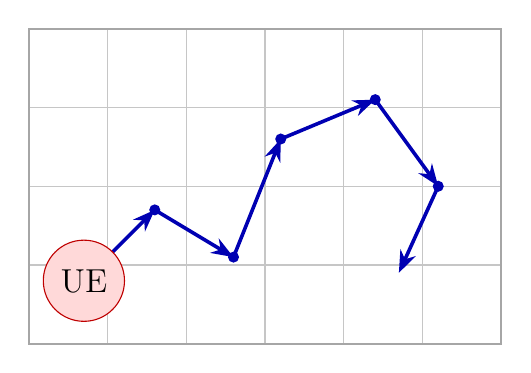
\begin{tikzpicture}[
    pathline/.style={-{Stealth[scale=0.9]}, blue!70!black, line width=1.3pt},
    point/.style={circle, fill=blue!70!black, minimum size=4pt, inner sep=0pt},
    ue/.style={circle, draw=red!75!black, fill=red!15, minimum size=7mm}
]
\draw[gray!45, step=1.0] (0,0) grid (6,4);
\draw[thick, gray!70] (0,0) rectangle (6,4);
\coordinate (p0) at (0.7,0.8);
\coordinate (p1) at (1.6,1.7);
\coordinate (p2) at (2.6,1.1);
\coordinate (p3) at (3.2,2.6);
\coordinate (p4) at (4.4,3.1);
\coordinate (p5) at (5.2,2.0);
\coordinate (p6) at (4.7,0.9);
\draw[pathline] (p0) -- (p1);
\draw[pathline] (p1) -- (p2);
\draw[pathline] (p2) -- (p3);
\draw[pathline] (p3) -- (p4);
\draw[pathline] (p4) -- (p5);
\draw[pathline] (p5) -- (p6);
\foreach \p in {p0,p1,p2,p3,p4,p5}
    \node[point] at (\p) {};
\node[ue] at (p0) {\small UE};
\end{tikzpicture}
\caption{Example of UE movement in the Random Walk mobility model}
\label{fig:random-walk-mobility}
\end{figure}

In this thesis, the Random Walk model is introduced only as a reference mobility model. It is not used as the main movement model because it does not represent lane-like or street-grid constraints. The implemented UE movement follows the Manhattan mobility model, which is more appropriate for studying radio measurements in a structured urban deployment.

The Manhattan mobility model is a geographic-restriction mobility model designed to represent movement on an urban street grid \cite{bai2003}. The service area is divided into horizontal and vertical road segments that form an orthogonal grid. A UE moves only along these road segments and may travel in one of four directions: East, North, West, or South. Direction changes are permitted at intersections, where the UE may continue forward or select another valid road while remaining inside the service area.

\begin{figure}[H]
\centering
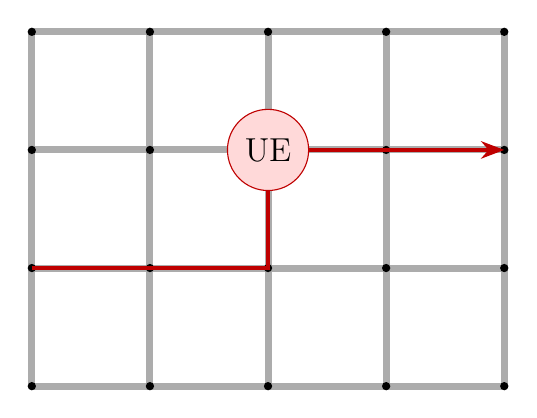
\begin{tikzpicture}[
    road/.style={gray!65, line width=2.5pt},
    route/.style={-{Stealth[scale=0.9]}, red!75!black, line width=1.4pt},
    intersection/.style={circle, fill=black, minimum size=3pt, inner sep=0pt}
]
\foreach \x in {0,1.5,3,4.5,6}
    \draw[road] (\x,0) -- (\x,4.5);
\foreach \y in {0,1.5,3,4.5}
    \draw[road] (0,\y) -- (6,\y);
\foreach \x in {0,1.5,3,4.5,6}
    \foreach \y in {0,1.5,3,4.5}
        \node[intersection] at (\x,\y) {};
\draw[route] (0,1.5) -- (3,1.5) -- (3,3) -- (6,3);
\node[circle, draw=red!75!black, fill=red!15, minimum size=7mm] at (3,3) {\small UE};
\end{tikzpicture}
\caption{Example of UE movement in a Manhattan street grid}
\label{fig:manhattan-mobility}
\end{figure}

In the implemented simulator, the road grid is constructed from vertical and horizontal line sets over the rectangular study area. The distance between adjacent road lines is entered as a simulation parameter. Each UE begins at one of the generated road intersections, so its initial position already satisfies the Manhattan-grid constraint. At an intersection, the available movement directions are determined by the remaining road segments inside the rectangle. This prevents the UE from selecting a direction that would immediately leave the study area.

UE movement is continuous along each road segment. During one simulation interval, the nominal travel distance is determined by the base UE speed and the duration of the time step:

\begin{equation}
    d_{\mathrm{move}} = v \Delta t,
\end{equation}

where \(d_{\mathrm{move}}\) is the nominal distance traveled during one time step, \(v\) is the base UE speed, and \(\Delta t\) is the time-step duration. The base speed is sampled once for each UE from the height-dependent speed interval selected for the scenario height. Therefore, UEs in the same simulation run share the same altitude but may have different sampled speeds. This is useful for multi-UE simulations because the dataset can contain several independent trajectories under the same altitude condition.

The effective movement distance can be reduced by the stop-and-go mechanism. Let \(\alpha_k\) denote the speed factor at time step \(k\), where \(0\le\alpha_k\le1\). The distance applied to the UE position update is

\begin{equation}
    d_{\mathrm{eff}}(k)=\alpha_k v\Delta t.
\end{equation}

When the UE is moving normally, \(\alpha_k=1\). When the UE is stopped, \(\alpha_k=0\). During the acceleration phase after a stop, \(\alpha_k\) increases gradually until the UE returns to its base speed. In the current simulation setting, after three direction changes the UE pauses for nine steps and then ramps up over two steps. This mechanism is not a full traffic-flow model, but it prevents the mobility trace from becoming an unrealistically constant-speed sequence and creates more varied radio-measurement behavior near intersections.

For a movement direction \(u_k\in\{\mathrm{E},\mathrm{N},\mathrm{W},\mathrm{S}\}\), the position update follows the road axis rather than an arbitrary angle:

\begin{equation}
    (x_{k+1},y_{k+1}) =
    \begin{cases}
    (x_k+d_{\mathrm{eff}}(k),y_k), & u_k=\mathrm{E},\\
    (x_k,y_k+d_{\mathrm{eff}}(k)), & u_k=\mathrm{N},\\
    (x_k-d_{\mathrm{eff}}(k),y_k), & u_k=\mathrm{W},\\
    (x_k,y_k-d_{\mathrm{eff}}(k)), & u_k=\mathrm{S}.
    \end{cases}
\end{equation}

When the remaining distance in the current time step is larger than the distance to the next intersection, the UE first reaches that intersection, selects a valid outgoing road, and then continues moving with the remaining distance. This detail is important because it allows one simulation step to cross an intersection without losing distance, while still enforcing the Manhattan-grid constraint.

The Manhattan update procedure can be summarized as follows:

\begin{enumerate}
    \item initialize each UE at a random road-grid intersection;
    \item assign an initial valid direction from the available cardinal directions;
    \item compute the effective travel distance for the current step;
    \item move the UE along the current road segment until the distance is exhausted or an intersection is reached;
    \item at an intersection, randomly select one valid direction and update the turn counter if the direction changes;
    \item trigger a pause and ramp-up cycle after the configured number of direction changes.
\end{enumerate}

This mobility model is especially relevant to the radio-measurement objective of the thesis. As the UE moves along the street grid, its distance and relative direction to surrounding gNBs change over time. These changes affect LOS probability, path loss, shadow fading, RSRP, interference, and SINR. When a neighboring gNB becomes stronger than the current serving gNB by more than the handover margin, the serving-cell index changes and a handover flag is recorded in the dataset. Thus, the combination of the hexagonal gNB layout and Manhattan mobility provides a consistent geometric foundation for studying radio-measurement variation and HO-related serving-cell behavior.

\subsection{Implementation of Handover Procedure in StormSIM}

\textcolor{red}{Contents: i) 3gpp handover procedure (figures and description); ii) implementation in StormSIM; iii) evaluation metrics of HO performance: pingpong, radio failure.... - detail descprition }


StormSim communicates with the free5GC AMF through SCTP/NGAP on N2 and supports GTP-U on N3. Loss is temporarily disabled while the UE registers and establishes a PDU session, then restored for the handover experiment.

Measurement mode reads \texttt{Step}, \texttt{connected\_gnb}, \texttt{gnbX\_rsrp}, and optional \texttt{Type}. A normal trigger occurs when \texttt{connected\_gnb} changes. The handover monitor follows

\begin{equation}
\mathrm{NULL}\rightarrow\mathrm{PREPARE}\rightarrow\mathrm{EXECUTE}
\rightarrow\mathrm{COMPLETE}\rightarrow\{\mathrm{SUCCESS},\mathrm{FAIL}\}.
\end{equation}

YAML parameters independently configure packet loss, one-way latency, and jitter for radio and Xn paths.

\begin{table}[H]
\centering
\caption{Implemented handover timers}
\begin{tabular}{lrlr}
\toprule
Timer & Value & Timer & Value\\
\midrule
TXnRELOCprep & 3 s & TXnRELOCoverall & 6 s\\
TNGRELOCprep & 5 s & TNGRELOCoverall & 10 s\\
T304 & 1000 ms & T310 & 1 s\\
T311 & 3 s & T301 & 2 s\\
T312 & 500 ms & T430 & 30 s\\
\bottomrule
\end{tabular}
\end{table}

The test plan states T304 = 100 ms, but executable source defines 1000 ms.

\textbf{TODO: cần xác nhận từ người dùng.} Confirm the official T304 value.

In addition, the current Xn trigger explicitly assigns the new virtual radio connection a downlink execution delay equal to T304 plus 500 ms. This setting is intended to exercise T304 failure behavior. It does not match archived successful timer records that stop T304 after only tens of milliseconds.

\textbf{TODO: cần xác nhận từ người dùng.} Identify the exact source revision and command used for each official archived result.



\subsubsection{Evaluation Metrics}

The authoritative trial output records source, target, handover type, result, failure reason, and total procedure time. The metrics are success rate, failure rate, and successful-trial mean, median, and 95th-percentile delay. The log column named \texttt{pdr} currently stores \texttt{PacketLoss}; it is interpreted as loss probability in this report.

\subsection{Chapter Conclusion}

This chapter described the system design used in the thesis. It presented the radio simulation workflow, the handover-emulation workflow, the measurement-driven trigger mechanism, the recorded output fields, and the metrics used for delay and success analysis. The design also separates radio-level serving-cell behavior from protocol-level handover execution, which is necessary for interpreting the results correctly. The next chapter uses the available generated data and experiment logs to evaluate radio behavior, handover success, delay, timer behavior, and current experimental limitations.

\pagebreak 

\section*{CHAPTER 4. EXPERIMENTAL RESULTS}
\addcontentsline{toc}{section}{\protect\numberline{}CHAPTER 4. EXPERIMENTAL RESULTS}
\setcounter{section}{4}
\setcounter{subsection}{0}
\setcounter{figure}{0}
\setcounter{table}{0}
\subsection{Experimental Scenarios}

\textcolor{red}{Contents: i) objectives of test; ii) test scenario description: table of setting parameters for A2G; mobility of ue, number ue, number of test repetition (for statistically correct); iii) how to measure the evaluation metrics}
\subsubsection{Experiment Objectives}

The first objective is to evaluate the effect of UE/UAV altitude on the generated radio measurements. A higher aerial UE may have a higher probability of LOS connection to several gNBs, which can improve the serving-link received power but can also increase interference from neighboring cells. Therefore, altitude is expected to affect RSRP and SINR in different ways.

The second objective is to evaluate mobility and handover behavior. The simulator records the serving BS, neighboring-cell RSRP values, UE velocity, and handover indicators. These outputs make it possible to identify when the serving BS changes, where handover events occur along the trajectory, and whether the number of handovers changes across altitude ranges.

The third objective is to evaluate protocol-level handover delay under selected delay and loss settings. This part uses handover-emulation logs to measure completion time, timeout behavior, and failure cases. The purpose is not to merge radio measurement and protocol delay into one metric, but to compare the radio-level trigger behavior with the protocol-level execution behavior.

\subsubsection{Altitude-Range Design}

The altitude cases are grouped by height intervals rather than by a single fixed UAV height. This design follows the height regimes used by the propagation models in Chapter 2 and Chapter 3. In the 3GPP UMa model, low-height terrestrial UE modelling is used for \(1.5\le h_{\mathrm{UE}}\le22.5\) m. The height-correction term in the LOS-probability expression becomes active above 13 m. For aerial vehicles, 3GPP TR 36.777 extends the UMa model to UMa-AV conditions for \(22.5<h_{\mathrm{UE}}\le300\) m, with the implemented aerial NLOS expression used up to 100 m and a LOS-dominant high-altitude branch above 100 m \cite{3gpp_38901,3gpp_36777}.

\begin{table}[H]
\centering
\caption{Altitude ranges used for A2G radio-measurement experiments}
\small
\renewcommand{\arraystretch}{1.12}
\begin{tabularx}{\textwidth}{p{2.2cm}p{3.2cm}X}
\toprule
Range & Height interval & Model interpretation\\
\midrule
H0 & \(1.5\le h_{\mathrm{UE}}\le13\) m & Ground or low terrestrial UE range under the UMa model.\\
\addlinespace[2pt]
H1 & \(13<h_{\mathrm{UE}}\le22.5\) m & Elevated terrestrial or low-height UE range under the UMa model.\\
\addlinespace[2pt]
H2 & \(22.5<h_{\mathrm{UE}}\le100\) m & Low-to-medium aerial UE range under the UMa-AV model.\\
\addlinespace[2pt]
H3 & \(100<h_{\mathrm{UE}}\le300\) m & High aerial UE range under the UMa-AV model.\\
\bottomrule
\end{tabularx}
\renewcommand{\arraystretch}{1.0}
\label{tab:altitude-ranges-a2g}
\end{table}

The main A2G comparison uses H2 and H3, because these ranges represent aerial UE operation. H0 is kept as the terrestrial baseline, and H1 is kept as a transition range between ordinary ground-level operation and aerial operation. When detailed plots are produced, one representative height may be selected from each range for time-series visualization, while repeated runs within the same range are used for aggregate statistics.

\subsubsection{Scenario Description}

\begin{table}[H]
\centering
\caption{Experimental scenario groups}
\small
\begin{tabularx}{\textwidth}{p{1.7cm}X X}
\toprule
Scenario & Description & Purpose\\
\midrule
S1 & Baseline terrestrial and low-height UE scenario using H0 and H1. & Provide a reference for comparing aerial UE radio behavior.\\
\addlinespace[2pt]
S2 & A2G scenario with different altitude ranges using H2 and H3. & Analyze the impact of UAV altitude on RSRP, SINR, shadow fading, serving-cell changes, and handover indicators.\\
\addlinespace[2pt]
S3 & A2G scenario with different handover-delay or transport-delay settings. & Analyze the impact of delay on handover completion time, timeout cases, and failure behavior.\\
\bottomrule
\end{tabularx}
\label{tab:experimental-scenario-groups}
\end{table}

The radio simulation settings are kept fixed across altitude scenarios except for UE height. This makes the altitude effect easier to interpret because the carrier frequency, gNB transmit power, antenna gains, bandwidth, noise figure, handover margin, and mobility model remain unchanged.

\begin{table}[H]
\centering
\caption{Main simulation settings for A2G experiments}
\small
\begin{tabularx}{\textwidth}{p{4.0cm}p{3.4cm}X}
\toprule
Parameter & Value & Role in the experiment\\
\midrule
Carrier frequency & 2 GHz & Used in path-loss calculation\\
gNB transmit power & 46 dBm & Downlink link-budget parameter\\
gNB antenna gain / UE antenna gain & 2 dB / 0 dB & Used in received-power calculation\\
gNB antenna height & 25 m & Ground gNB height\\
UE height & Ranges H0--H3 & Main variable in altitude scenarios\\
Bandwidth / UE noise figure & 10 MHz / 9 dB & Used in thermal-noise calculation\\
Handover margin & 3 dB & RSRP-based serving-cell change condition\\
Mobility model & Manhattan mobility & UE moves along an urban road grid\\
UE speed & 20--60 km/h & Randomly assigned by the simulator\\
Simulation duration & 300 steps & One-second output interval\\
Number of UEs & 1 for trace plots; multiple UEs for aggregate runs & Controls whether the result is trajectory-level or aggregate-level\\
Repetitions & 30 runs per scenario & Reduces randomness from mobility, LOS/NLOS sampling, and shadow fading\\
\bottomrule
\end{tabularx}
\label{tab:a2g-simulation-settings}
\end{table}

For statistically meaningful comparison, each scenario should be repeated with different random seeds or independently generated UE trajectories. In this thesis, 30 repetitions per scenario are planned as the default setting. If execution time is limited, at least 10 repetitions can be used for preliminary analysis, but final comparison should report the number of repetitions explicitly.

\subsubsection{Evaluation Metrics}

The radio-level metrics are extracted from the simulator CSV output. RSRP is used to evaluate serving-cell and neighboring-cell signal strength. SINR is used to evaluate link quality under interference and thermal noise. Shadow fading is used to observe slow large-scale signal variation. UE velocity is used to interpret how fast the radio condition changes along the trajectory. The serving BS index and handover flag are used to identify cell changes and handover events.

For each scenario, the evaluation includes both time-series and scenario-level statistics. Time-series plots show how RSRP, SINR, shadow fading, speed, and serving BS evolve along one representative UE trajectory. Scenario-level plots compare the distribution or average value of RSRP, SINR, and number of handovers across altitude ranges or delay settings. The handover-related metrics include the number of handovers, handover event time, source and target BS, success rate, failure rate, and successful-trial handover delay when protocol-level logs are available.

\subsection{Radio Measurement Results}

This subsection reports the radio measurements generated by the simulator. The main plotted metrics are RSRP, SINR, shadow fading, and UE velocity. These metrics are analyzed together because they describe different parts of the same radio condition. RSRP mainly represents the received strength of the serving or neighboring cell, SINR represents the useful-signal quality after interference and noise are considered, shadow fading represents slow random variation around the median path loss, and velocity explains how quickly the UE moves through changing radio conditions.

The result presentation should include the following figures after the official simulation runs are generated:

\begin{itemize}
    \item RSRP over time for representative altitude ranges;
    \item SINR over time for representative altitude ranges;
    \item shadow fading over time for the serving link;
    \item UE velocity over time;
    \item RSRP comparison across altitude ranges;
    \item SINR comparison across altitude ranges.
\end{itemize}

When the UE moves farther from the serving gNB, the received signal strength generally decreases, which leads to a lower RSRP. However, RSRP is not determined only by distance. The LOS/NLOS state and shadow fading can also change the received power, so the RSRP curve may fluctuate even when the UE trajectory is smooth.

SINR can vary differently from RSRP because it depends on the serving-cell received power, neighboring-cell interference, and thermal noise. In aerial scenarios, a higher UE altitude may increase LOS visibility to the serving gNB, but it may also increase visibility to neighboring gNBs. Therefore, an altitude range with stronger RSRP does not always produce better SINR. Near cell-edge regions, or when several neighboring gNBs are received strongly, SINR may decrease even if the serving-cell RSRP remains acceptable.

Shadow fading explains slow signal variation caused by environmental obstruction and large-scale propagation randomness. In the simulator, the shadow-fading value is cached per UE--gNB link and updated after a movement distance threshold. As a result, shadow fading changes more slowly than instantaneous geometry-based received power and can create signal fluctuation even when the UE movement does not change abruptly.

Velocity is included to support interpretation of the radio time series. A faster UE moves through serving-cell and neighboring-cell regions more quickly, so RSRP and SINR may change more rapidly and handover opportunities may appear closer together in time. The velocity curve is therefore useful when explaining whether radio-measurement changes are caused by propagation conditions alone or by rapid movement through the cellular layout.

\subsection{Handover Behavior Analysis}

The radio simulator identifies handover events from serving-BS changes. A handover indicator is recorded when the selected serving BS differs from the previous serving BS. This radio-level handover event should be interpreted as a serving-cell transition suggested by the measurement model, not as a completed protocol-level handover procedure.

The handover behavior should be evaluated using the following outputs:

\begin{itemize}
    \item serving BS over time;
    \item handover event timeline;
    \item number of handovers per altitude range;
    \item source and target BS for each handover event;
    \item UE position and speed at each handover event;
    \item comparison between handover count and altitude range.
\end{itemize}

Handover events are expected to occur mainly when the UE moves toward the boundary between two cells. In this region, the RSRP of a neighboring gNB may become higher than the RSRP of the current serving gNB by more than the configured handover margin. A higher speed can make these transitions occur over fewer simulation steps, while a higher altitude can change the number of visible candidate gNBs and the interference condition. Therefore, the handover analysis should be interpreted together with the RSRP, SINR, and velocity plots rather than from the handover count alone.

For protocol-level delay analysis, the handover-emulation results are evaluated separately using trial-summary and timer-event logs. The main metrics are success rate, failure rate, timeout cases, mean successful handover delay, median successful handover delay, and 95th-percentile successful handover delay. This separation preserves the distinction between a radio-level serving-cell change and the completion of the actual handover signaling procedure.

\subsection{Validation Scope}

The handover-delay results in this chapter are obtained from StormSim trial-summary CSV files and timer-event logs generated while StormSim interacts with the free5GC core network. The repository contains many development logs but no single clearly labeled complete factorial experiment. Two large Xn runs with a logged one-way delay parameter of 20 ms are used for the verified comparison. Because the \texttt{pdr} field is populated from \texttt{PacketLoss}, its values are interpreted as loss probabilities.

\begin{table}[H]
\centering
\caption{Verified handover summaries}
\begin{tabular}{lrrrrr}
\toprule
Run & Loss & Trials & Success & Failure & Rate\\
\midrule
1781614531 & 0.10 & 210 & 210 & 0 & 100.00\%\\
1781622441 & 0.50 & 195 & 171 & 24 & 87.69\%\\
\bottomrule
\end{tabular}
\end{table}

\textbf{TODO:} Confirm that these are official rather than debugging runs.

\begin{figure}[H]
\centering
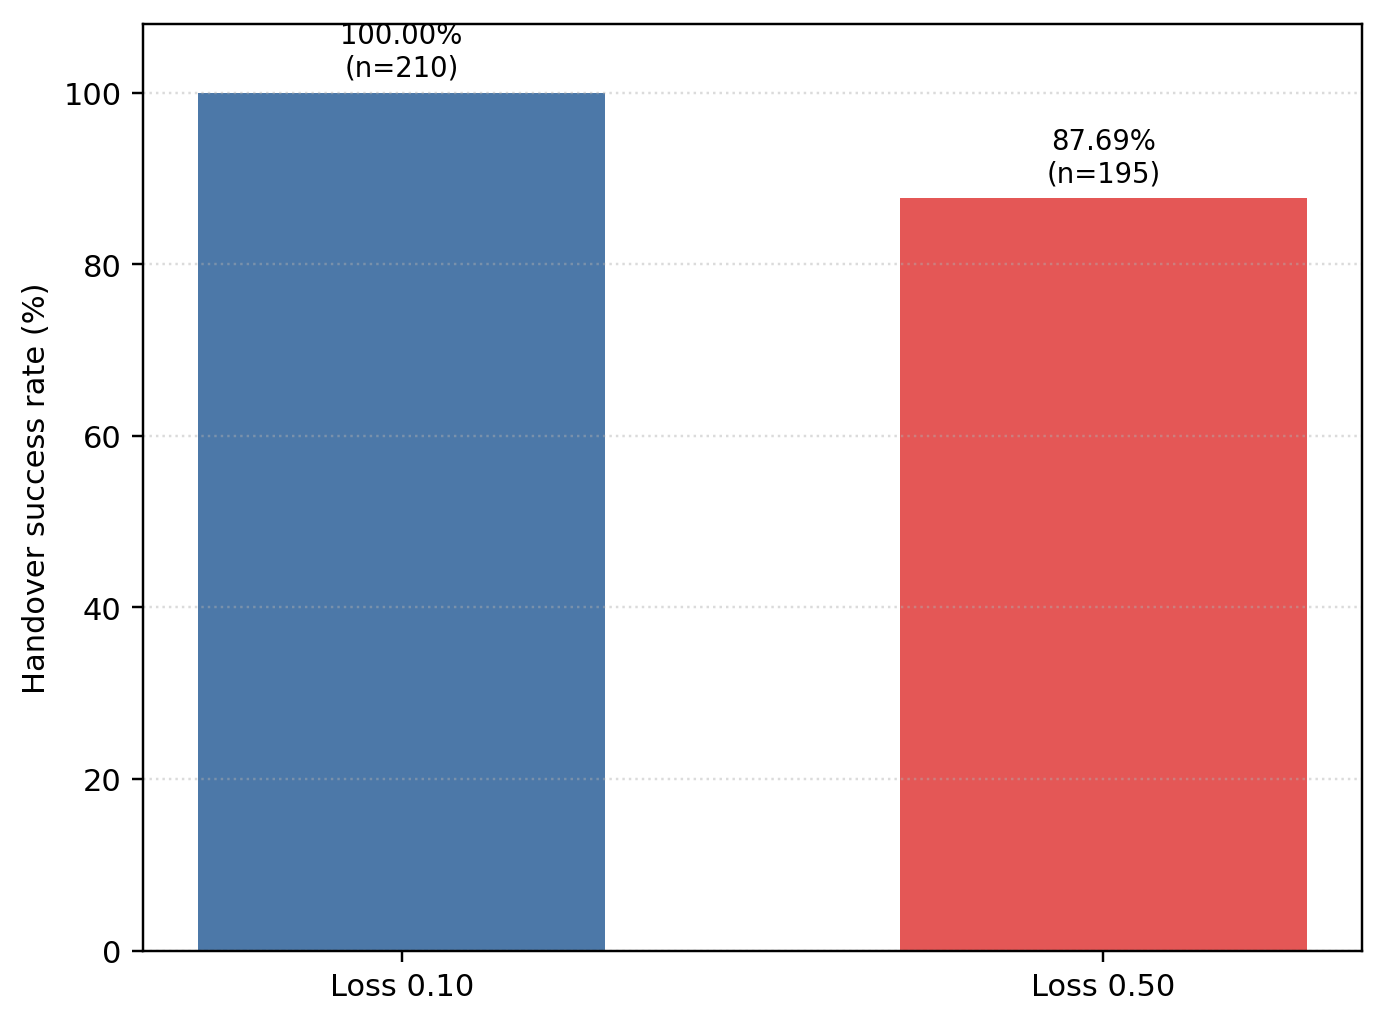
\includegraphics[width=0.82\textwidth]{Images/archived_ho_success_rate.png}
\caption{Handover success rate reproduced from the two archived trial-summary files}
\label{fig:archived-ho-success}
\end{figure}

Figure~\ref{fig:archived-ho-success} is descriptive rather than a controlled loss-response curve. The runs have different archived trial counts, and the exact source revision is unknown.

\subsection{Handover Success and Delay}

At loss 0.10, all 210 attempts succeeded. At loss 0.50, 171 of 195 succeeded; all 24 failures were labeled \texttt{Timeout}. The matching timer file contains 24 Xn preparation transport failures, 24 preparation timeouts, and 24 overall cancellations, associating these failures with unsuccessful Xn preparation.

\begin{figure}[H]
\centering
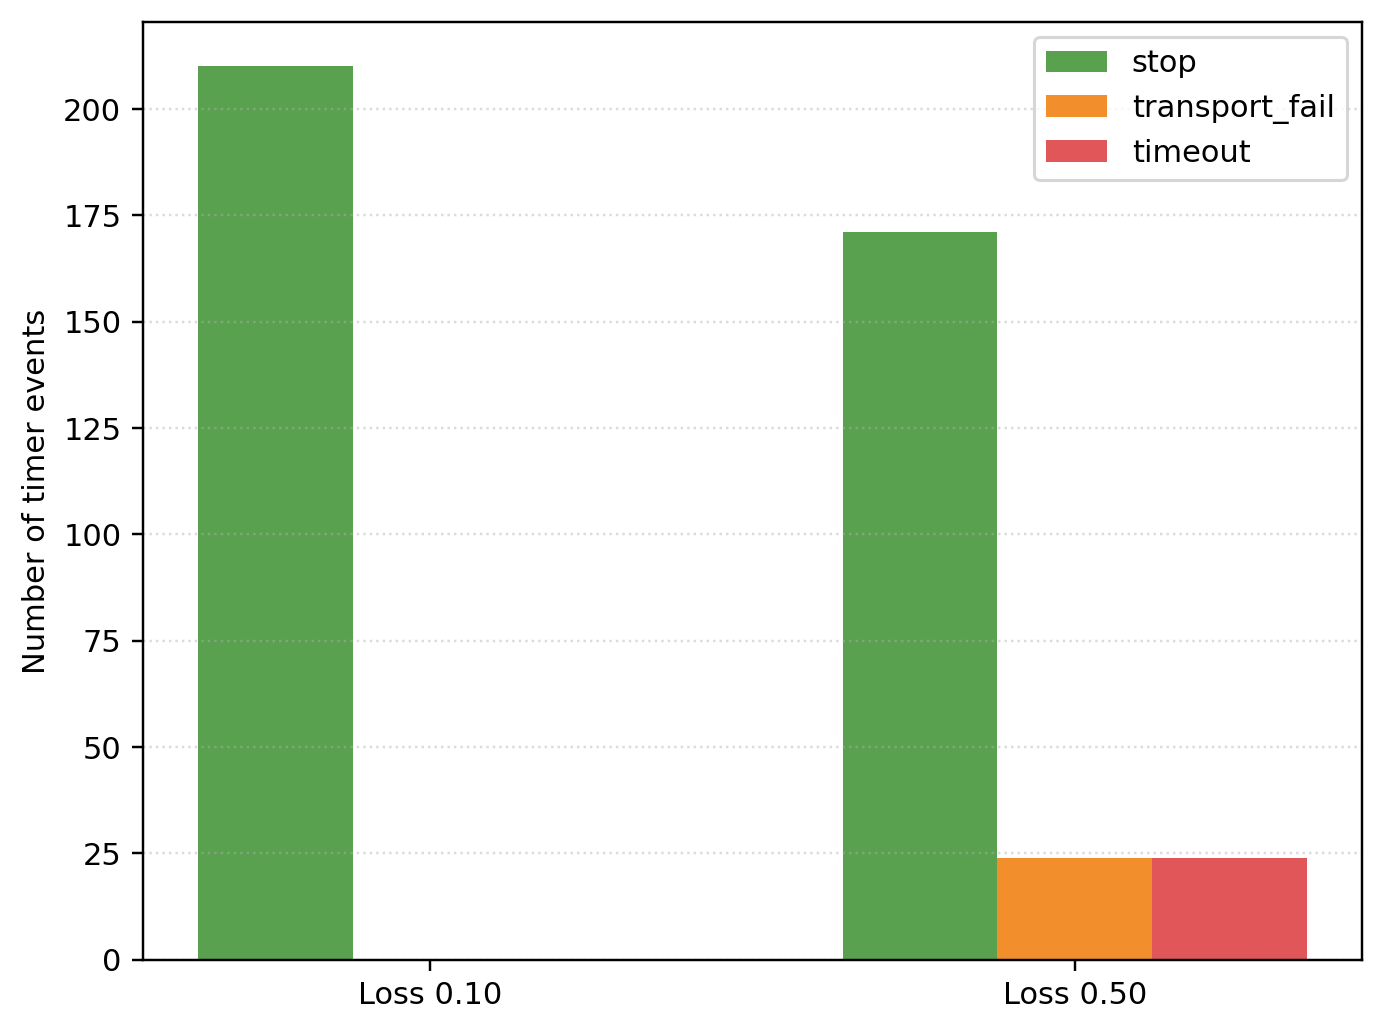
\includegraphics[width=0.82\textwidth]{Images/archived_xn_prep_outcomes.png}
\caption{TXnRELOCprep terminal and diagnostic events in the archived timer files}
\label{fig:archived-xn-prep}
\end{figure}

The \texttt{transport\_fail} and \texttt{timeout} bars at loss 0.50 describe the same 24 failed preparation lifecycles at different points: context forwarding first reports a transport failure, while the preparation timer is intentionally left active and later expires. They must not be added as 48 independent failed handovers.

\begin{table}[H]
\centering
\caption{Successful Xn handover delay}
\begin{tabular}{lrrr}
\toprule
Loss & Mean & Median & 95th percentile\\
\midrule
0.10 & 200.597 ms & 200.574 ms & 201.061 ms\\
0.50 & 200.627 ms & 200.628 ms & 201.062 ms\\
\bottomrule
\end{tabular}
\end{table}

Successful durations cluster around 200.6 ms because the scenario polls completion every 200 ms. The value is therefore quantized and is not a precise lower-layer latency measurement.

\begin{figure}[H]
\centering
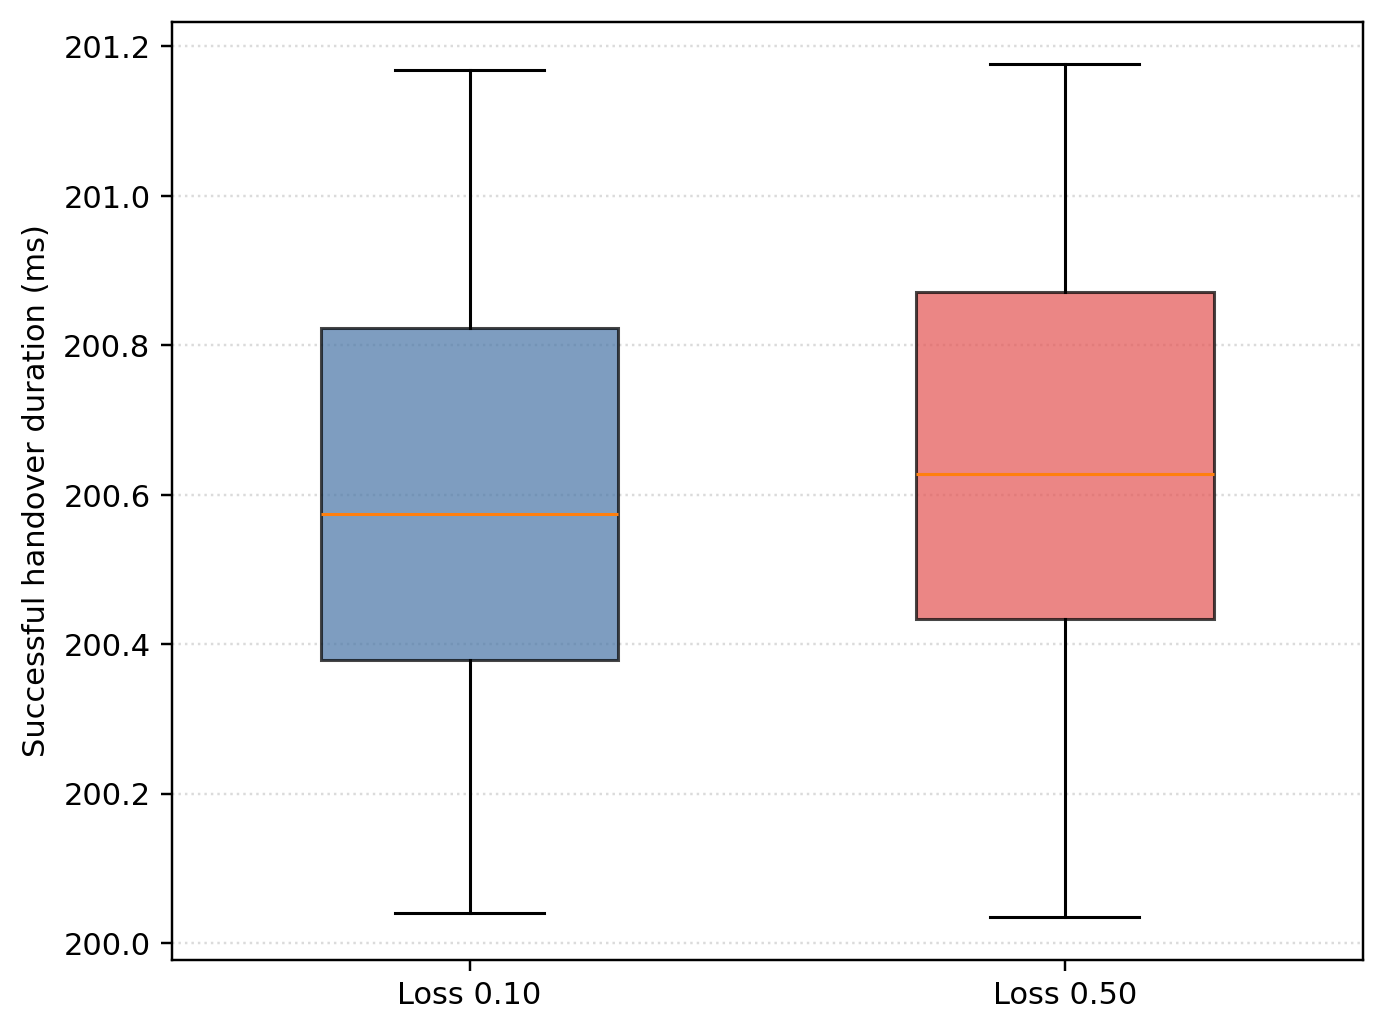
\includegraphics[width=0.82\textwidth]{Images/archived_ho_delay_boxplot.png}
\caption{Distribution of successful handover durations in the archived trial summaries}
\label{fig:archived-ho-delay}
\end{figure}

The narrow boxes in Fig.~\ref{fig:archived-ho-delay} do not demonstrate intrinsically low protocol jitter. They mainly show that the outer scenario observes completion at a 200 ms polling boundary.

\subsection{Timer Consistency and Missing Scenarios}

Raw timer coverage is incomplete. Run 1781614531 has 210 successful summaries but only 50 terminal T304 records, including one T304 timeout despite no failed trial. Trial summaries are therefore used as the authoritative overall outcome; T304 timeout rates are not reported.

The source supports several planned experiment outputs: loss--delay evaluation, a T304 breakpoint search, an RLF cascade, an Xn/N2 comparison, and beam-failure analysis. However, the repository does not contain a clearly labeled complete result set for all scenarios. RLF, beam, and N2 RTT fields are generally empty or zero.

There is also evidence that the archived logs were not generated by the exact current source state. The current Xn trigger sets the handover connection delay to T304 plus 500 ms, which should deliberately exceed T304, whereas archived successful records show T304 stopping after tens of milliseconds. The archived statistics are valid descriptions of those CSV files, but they cannot yet be claimed as reproducible results of the current executable revision.

\textbf{TODO:} Identify the archived source revision, then repeat the official timer campaign after fixing T304 and timer lifecycle coverage.

\subsection{Chapter Conclusion}

This chapter defined the experimental scenario groups for radio-measurement and handover-delay analysis. The altitude design follows the height regimes used by the UMa and UMa-AV propagation models, so the A2G experiments can compare terrestrial, transition, low-to-medium aerial, and high-aerial UE behavior. The chapter also described the planned radio-measurement plots and the metrics used to interpret RSRP, SINR, shadow fading, velocity, serving-cell changes, and handover events. The verified archived Xn runs demonstrate measurement-driven handover execution and show reduced success under higher signaling loss, while the delay results reveal polling quantization and timer-telemetry limitations. The next chapter summarizes the thesis, states the main limitations, and outlines future work.

\pagebreak 

\section*{CHAPTER 5. CONCLUSION}
\addcontentsline{toc}{section}{\protect\numberline{}CHAPTER 5. CONCLUSION}
\setcounter{section}{5}
\setcounter{subsection}{0}
\setcounter{figure}{0}
\setcounter{table}{0}
\subsection{Summary and Contributions}

This thesis developed a workflow for studying 5G mobility from two complementary viewpoints: radio-level measurement behavior and protocol-level handover execution. The Python radio simulator generates structured mobility and radio-measurement traces, including UE position, UE height, serving-cell information, RSRP, SINR, shadow fading, and handover indicators. The StormSim-based emulation workflow then replays measurement-driven serving-cell changes in a free5GC environment and records handover trial summaries and timer events.

The main contribution of the thesis is the separation between a radio-level serving-cell change and a completed protocol-level handover. In the radio simulator, a handover indicator means that the selected serving gNB changes according to an RSRP-based rule. In StormSim, the handover is treated as a protocol procedure involving source gNB, target gNB, UE context transfer, path switch, T304, and Xn relocation timers. This separation avoids treating a measurement decision as if it were already a completed handover.

A second contribution is the construction of a structured radio-data generation pipeline for terrestrial and aerial UE-height ranges. The simulator supports UMa and UMa-AV propagation behavior, height-dependent mobility settings, hexagonal gNB placement, and CSV output suitable for post-processing. A third contribution is the creation of a StormSim-ready seven-gNB measurement trace with fixed gNB-indexed RSRP columns, allowing the generated radio data to be replayed by the handover emulator without losing the identity of each gNB.

\subsection{Main Findings}

The radio-measurement results show that UE height has different effects on RSRP and SINR. Compared with the terrestrial height ranges, the aerial height ranges produce stronger average serving-cell RSRP because the UE has more favorable propagation and a higher probability of LOS connection. However, the SINR does not improve in the same way. At aerial heights, the UE can also receive stronger signals from neighbouring gNBs, so co-channel interference increases. As a result, the average SINR decreases in the H2 and H3 altitude ranges even though the serving-cell RSRP is higher. This confirms that RSRP alone is not sufficient for evaluating A2G mobility quality.

The generated radio traces also show that shadow fading introduces slow signal variation around the path-loss trend. The shadow-fading distribution becomes narrower at higher altitude, especially in the H3 range. This behavior is consistent with the implemented height-dependent propagation model and helps explain why aerial traces can have stronger but more interference-limited received signals.

For protocol-level evaluation, a seven-gNB measurement trace was generated with one center gNB and six surrounding first-tier gNBs. The trace contains 301 measurement steps and 18 serving-cell changes. When replayed in StormSim as Xn handover opportunities under the baseline no-loss condition, all 18 handover trials completed successfully. The successful trial-summary delay has a mean of 200.530 ms, a median of 200.550 ms, and a 95th percentile of 201.013 ms.

The timer-event log provides a finer interpretation of this delay. In the same run, \texttt{T304} stopped successfully for all 18 handovers with an average elapsed time of 10.621 ms, while \texttt{TXnRELOCprep} and \texttt{TXnRELOCoverall} stopped within about 1 ms on average. Therefore, the approximately 200 ms trial-summary delay mainly reflects the scenario-level polling interval used to observe handover completion, not the duration of every internal protocol phase.

\subsection{Limitations}

The radio simulator is a controlled system-level model rather than a full physical-layer implementation. RSRP is derived from received power using a resource-grid approximation, and the serving-cell decision uses an RSRP margin without time-to-trigger, measurement filtering, or full RRC measurement-event processing. The LOS/NLOS state and shadow fading are cached per UE--gNB link to keep the trace spatially stable, but this remains an abstraction of real propagation dynamics.

The current StormSim result is a baseline validation of the measurement-driven workflow, not a complete performance study under all network conditions. The verified seven-gNB run uses Xn handover with zero packet loss, zero added latency, and zero jitter. It demonstrates that the generated measurement trace can drive successful protocol-level handovers, but it does not yet quantify handover robustness under degraded transport conditions.

The trial-summary delay is also affected by the implementation of the scenario runner. Completion is checked using a 200 ms polling ticker, so the exported successful handover duration is quantized around 200 ms. Timer-event logs are therefore necessary when interpreting lower-level handover phases. In addition, the CSV interface between the Python simulator and StormSim still requires a dedicated adapter script for fixed gNB-indexed RSRP columns.

Finally, the present evaluation focuses on Xn handover. N2 handover, full CHO mode evaluation, RLF behavior, beam-failure behavior, and systematic loss--delay experiments remain outside the verified result set reported in this thesis.

\subsection{Future Work}

Future work should first unify the radio-simulator and StormSim CSV formats so that fixed gNB-indexed RSRP fields are produced directly by the main simulator logger. This would remove the need for a separate adapter script and make measurement-driven handover experiments easier to reproduce.

The handover-delay evaluation should then be extended from the baseline no-loss case to a controlled matrix of packet loss, latency, and jitter settings. This matrix should report success rate, failure reason, timeout behavior, mean delay, median delay, and percentile delay for each setting. Xn and N2 handover should also be compared under the same measurement trace so that the effect of direct gNB-to-gNB handover and core-network-assisted handover can be separated.

Another important direction is to reduce or replace the 200 ms polling interval in the scenario runner. Event-driven completion logging would allow the trial-summary delay to better match the internal handover completion time. The timer lifecycle should also be checked so that each handover trial has complete and consistent start and terminal timer records.

On the radio side, future work can add time-to-trigger, measurement filtering, and additional RRC event conditions such as A5 to make the serving-cell and handover-trigger logic closer to real mobility procedures. The generated dataset can also be expanded to multiple UE trajectories and repeated fixed-seed scenarios to support more systematic statistical comparison.

\subsection{Chapter Conclusion}

This chapter summarized the thesis contributions, main findings, limitations, and future research directions. Overall, the thesis provides a practical platform for generating 5G mobility traces and analyzing handover behavior beyond simple serving-cell changes. The current results show that aerial UE height can improve RSRP while reducing SINR due to interference, and that a generated seven-gNB trace can drive successful Xn handovers in StormSim under baseline no-loss conditions. Broader claims about handover robustness require the controlled network-impairment and handover-type experiments described as future work.

\pagebreak 

\section*{APPENDIX A. IMPLEMENTATION AND DATA REFERENCE}
\addcontentsline{toc}{section}{\protect\numberline{}APPENDIX A. IMPLEMENTATION AND DATA REFERENCE}
\setcounter{section}{6}
\setcounter{subsection}{0}
\setcounter{figure}{0}
\setcounter{table}{0}

\subsection{Radio Simulator Module Mapping}

\begin{longtable}{p{3.2cm}p{10.7cm}}
\toprule
Module & Research responsibility\\
\midrule
\endfirsthead
\toprule
Module & Research responsibility\\
\midrule
\endhead
\texttt{main.py} & Reads scenario inputs and starts the interactive simulation.\\
\texttt{config.py} & Defines radio, mobility, timing, and output constants.\\
\texttt{hexagons.py} & Generates axial hexagonal gNB locations.\\
\texttt{mobility.py} & Implements roads, intersections, turns, boundaries, and stop-and-go motion.\\
\texttt{radio\_models.py} & Implements LOS probability, UMa/UMa-AV path loss, fading, RSRP, interference, SINR, and association.\\
\texttt{simulation.py} & Owns simulation state, executes each time step, updates visualization, and coordinates logging.\\
\texttt{logger.py} & Builds the per-step dataset and writes the combined CSV.\\
\texttt{ue.py} & Validates and stores aerial-UE metadata.\\
\texttt{utils.py} & Reads numeric input and applies defaults.\\
\bottomrule
\end{longtable}

\subsection{Protocol Test Environment}

\begin{longtable}{p{3.2cm}p{10.7cm}}
\toprule
Component & Research responsibility\\
\midrule
\endfirsthead
\toprule
Component & Research responsibility\\
\midrule
\endhead
\texttt{free5GC} & Provides the 5G Core functions used by the protocol-level experiment, especially AMF-side NGAP/N2 connectivity and user-plane support through GTP-U/N3.\\
\texttt{StormSim} & Emulates UE and gNB behavior for selected handover scenarios, connects to the 5G Core, injects configurable loss, delay, and jitter, and exports trial-summary and timer-event logs.\\
\texttt{Python radio simulator} & Generates radio-level mobility and measurement traces used to inspect RSRP, SINR, serving-cell changes, and neighbor-cell behavior.\\
\bottomrule
\end{longtable}

\subsection{StormSim Module Mapping}

\begin{longtable}{p{4.2cm}p{9.7cm}}
\toprule
Package & Research responsibility\\
\midrule
\endfirsthead
\toprule
Package & Research responsibility\\
\midrule
\endhead
\texttt{cmd/emulator} & Selects normal, replay, CSV, measurement, failure, and CHO modes.\\
\texttt{pkg/config} & Loads YAML and CSV input schemas.\\
\texttt{pkg/model} & Defines shared UE, gNB, session, event, RRC, and CHO data.\\
\texttt{internal/common/fsm} & Executes asynchronous state machines.\\
\texttt{internal/common/logger} & Records protocol, timer, delay, and CSV/NDJSON outputs.\\
\texttt{internal/transport/rlink} & Emulates UE--gNB channels with directional loss, delay, jitter, and counters.\\
\texttt{internal/transport/sctpngap} & Provides SCTP/NGAP transport to the AMF.\\
\texttt{internal/core/uecontext} & Implements UE 5GMM/5GSM, NAS security, sessions, handover execution, recovery timers, and CHO evaluation.\\
\texttt{internal/core/gnbcontext} & Implements gNB context, NGAP handling, Xn/N2 handover, path switch, and CHO preparation.\\
\texttt{internal/core/monitor} & Tracks handover phases, results, groups, NTN visibility metadata, and OAM responses.\\
\texttt{internal/scenarios} & Creates UE/gNB experiments and exports trial/timer results.\\
\texttt{monitoring} & Provides OAM, resource, PCAP, and GTP-U support.\\
\bottomrule
\end{longtable}

\subsection{Python Radio CSV Dictionary}

For UE index \(i\), the logger creates the following fields.

\begin{longtable}{p{4.6cm}p{9.3cm}}
\toprule
Column pattern & Meaning\\
\midrule
\endfirsthead
\toprule
Column pattern & Meaning\\
\midrule
\endhead
\texttt{Step} & Discrete simulation frame.\\
\texttt{ue\(i\)\_x}, \texttt{ue\(i\)\_y} & UE Cartesian position in metres.\\
\texttt{ue\(i\)\_height} & UE height above ground in metres.\\
\texttt{ue\(i\)\_direction} & 0: east, 1: north, 2: west, 3: south.\\
\texttt{ue\(i\)\_connected\_bs} & Serving gNB array index.\\
\texttt{ue\(i\)\_los\_probability} & Calculated LOS probability for the serving link.\\
\texttt{ue\(i\)\_los\_state} & Cached sampled state: LOS or NLOS.\\
\texttt{ue\(i\)\_pathloss} & Path loss before shadow fading, in dB.\\
\texttt{ue\(i\)\_shadow\_fading} & Additional shadow-fading loss, in dB.\\
\texttt{ue\(i\)\_rsrp} & Serving-cell RSRP approximation, in dBm.\\
\texttt{ue\(i\)\_prx} & Total serving received power, in dBm.\\
\texttt{ue\(i\)\_sinr} & Serving-link SINR, in dB.\\
\texttt{ue\(i\)\_speed} & Effective speed after pause/ramp factor, in km/h.\\
\texttt{ue\(i\)\_handover} & One if the serving index differs from the previous step.\\
\texttt{ue\(i\)\_bs\(n\)\_idx} & Index of ranked non-serving neighbor \(n\), \(1\leq n\leq6\).\\
\texttt{ue\(i\)\_bs\(n\)\_rsrp} & RSRP of that neighbor, in dBm.\\
\bottomrule
\end{longtable}

\subsection{StormSim Measurement Input Dictionary}

\begin{longtable}{p{4.3cm}p{9.6cm}}
\toprule
Column & Meaning\\
\midrule
\endfirsthead
\toprule
Column & Meaning\\
\midrule
\endhead
\texttt{Step} or \texttt{Bước} & Input sequence index.\\
\texttt{connected\_gnb} & Serving gNB identifier for the current row. A change creates a normal handover trigger.\\
\texttt{gnbX\_rsrp} & RSRP associated with gNB key \texttt{gnbX}; used by CHO or retained as measurement context.\\
\texttt{Type} & Handover type string; defaults to Xn when absent or empty.\\
\bottomrule
\end{longtable}

\subsection{Timer Event Output Dictionary}

\begin{longtable}{p{4.1cm}p{9.8cm}}
\toprule
Field & Meaning\\
\midrule
\endfirsthead
\toprule
Field & Meaning\\
\midrule
\endhead
\texttt{ts}, \texttt{start\_ts}, \texttt{stop\_ts} & Event and lifecycle timestamps.\\
\texttt{trial\_id} & Measurement-row/trial identifier.\\
\texttt{pdr} & Currently stores configured packet-loss probability despite its name.\\
\texttt{delay\_ms} & Configured delay copied into telemetry.\\
\texttt{ho\_type} & Xn or N2/NG label.\\
\texttt{timer\_name} & Timer whose lifecycle generated the event.\\
\texttt{event} & Start, stop, timeout, cancel, restart, zombie, or transport-failure marker.\\
\texttt{elapsed\_ms} & Duration measured by the timer engine.\\
\texttt{result}, \texttt{stop\_reason} & Interpreted terminal status.\\
\texttt{source\_gnb}, \texttt{target\_gnb} & Handover endpoints associated with the timer.\\
\texttt{rsrp\_at\_trigger} & Defined telemetry field; not populated in the selected logs.\\
\texttt{rlf\_detected}, beam/RLF/N2 fields & Defined for planned scenarios; zero or empty does not prove a measured zero.\\
\bottomrule
\end{longtable}

\subsection{Trial Summary Output Dictionary}

\begin{longtable}{p{4.1cm}p{9.8cm}}
\toprule
Field & Meaning\\
\midrule
\endfirsthead
\toprule
Field & Meaning\\
\midrule
\endhead
\texttt{trial\_id} & Handover attempt identifier.\\
\texttt{overall\_result} & \texttt{success} or \texttt{fail}.\\
\texttt{fail\_reason} & Scenario-level failure reason.\\
\texttt{total\_ho\_ms} & Time from monitor procedure start to observed completion/failure.\\
\texttt{source\_gnb}, \texttt{target\_gnb} & Source and requested target identifiers.\\
\texttt{pdr}, \texttt{delay\_ms}, \texttt{ho\_type} & Copied experiment-condition labels.\\
\texttt{rlf\_offset\_ms}, \texttt{rsrp\_during\_ho}, \texttt{reestab\_target\_gnb} & Planned RLF-scenario fields, generally unpopulated in the selected runs.\\
\bottomrule
\end{longtable}

\subsection{Reproducibility Checklist}

An official experiment package should retain:

\begin{enumerate}
    \item an immutable source revision;
    \item the exact command line and YAML configuration;
    \item the input measurement CSV and its schema version;
    \item all random seeds;
    \item timer values, especially T304;
    \item raw timer events and trial summaries;
    \item expected trial count and a timer-lifecycle completeness report;
    \item an explicit statement that \texttt{pdr} means loss probability or a corrected field name.
\end{enumerate}

\clearpage


\phantomsection
\addcontentsline{toc}{section}{\protect\numberline{}REFERENCES}
\bibliographystyle{IEEEtran}
\bibliography{references}










\end{document}
